\documentclass[12pt, oneside]{article}


% Pakete und Vorlagen einbinden
% Zusaetzliche Pakete

\usepackage[ngerman]{babel}
\usepackage{acronym}
\usepackage{enumerate}  
\usepackage{a4wide}
\usepackage{fancyhdr}
\usepackage{graphicx}
\usepackage{palatino}
\usepackage{float}
\usepackage{csquotes}
\usepackage[bookmarks, hidelinks]{hyperref}
\RequirePackage[ngerman=ngerman-x-latest]{hyphsubst}

\usepackage[style=authoryear-comp,dashed=false,natbib=true,backend=biber,maxnames=2]{biblatex}
\usepackage[justification=centering, labelfont=bf, textfont=bf]{caption}
\usepackage[a4paper, margin=0cm, left=3cm, top=2.5cm, right=2cm, bottom=3.5cm]{geometry} 
\usepackage{etoolbox}
\usepackage{acronym}
\usepackage{titlesec}
\usepackage[titles]{tocloft}
\usepackage{fontspec}
\usepackage[table,xcdraw]{xcolor}
\usepackage{pythonhighlighting}
\usepackage{minted}
\usepackage{wrapfig}


\definecolor{mygray}{rgb}{0.85,0.85,0.85}


\setminted[bash]{
	bgcolor=mygray,
	fontsize=\footnotesize,
	breaklines,
	breakafter=\_,
	breakafter=/,
	breaksymbolleft=,
	breakindent=15pt,
}



\setlength\cftparskip{-2pt}
\setlength\cftbeforesecskip{0pt}
\setlength\cftaftertoctitleskip{0pt}

%\setmainfont{Times New Roman}

\DeclareCaptionFormat{myformat}{\fontsize{10}{0}\selectfont#1#2#3}
\captionsetup{format=myformat}

\setlength\parindent{0pt}
\setlength{\parskip}{6pt}
\setlength{\headheight}{0.8cm}

\linespread{1.25}

%\setlength{\cftbeforesecskip}{1.75pt}

\renewcommand{\cftfigpresnum}{Abbildung }
\renewcommand{\cfttabpresnum}{Tabelle }

\renewcommand{\cftfigaftersnum}{:}
\renewcommand{\cfttabaftersnum}{:}

\setlength{\cftfignumwidth}{2.75cm}
\setlength{\cfttabnumwidth}{2cm}

\setlength{\cftfigindent}{0cm}
\setlength{\cfttabindent}{0cm}

\renewcommand{\figurename}{Abbildung}
\renewcommand{\tablename}{Tabelle}


%%%%%%%%%%%%%%%%%%%%%%%%%%%%%%
%% Definition der Kopfzeile %%
%%%%%%%%%%%%%%%%%%%%%%%%%%%%%%

\pagestyle{fancy}
\renewcommand{\headrulewidth}{0.5pt} %Linie oben
\renewcommand{\footrulewidth}{0.5pt} %Linie oben
\renewcommand{\sectionmark}[1]{\markboth{#1}{}}
\fancyhf{}
\headsep = 1cm
\fancyfoot[R]{\rule[+1.5ex]{0pt}{1ex}\thepage} %Kopfzeile rechts bzw. außen
\fancyfoot[L]{\nouppercase{\leftmark}}

%%%%%%%%%%%%%%%%%%%%%%%%%%%%%%%%%%%%%%%%%%%%%%%%%%%%%
%%  Definition des Deckblattes und der Titelseite  %%
%%%%%%%%%%%%%%%%%%%%%%%%%%%%%%%%%%%%%%%%%%%%%%%%%%%%%

\newcommand{\JMUTitle}[8]{
  \fancyhead[L]{\rule[-1.5ex]{0pt}{1ex} #2} %Kopfzeile links bzw. innen

  \thispagestyle{empty}
  
  
  
  \begin{center}
  	\includegraphics{Bilder/misc/thga_logo}\\
  	\vspace*{\stretch{1}}
    \Huge\bfseries
    #1\\
    \vspace*{\stretch{0.25}}
    \normalsize
    #3
  \end{center}

  \vspace*{\stretch{2}}

{\renewcommand{\arraystretch}{1.5}
\begin{tabular}{l l} 
    Eingereicht von:  & \hspace{4cm}#4\\ 
    Studiengang:  & \hspace{4cm}#6\\ 
    Matrikelnummer:  & \hspace{4cm}#8\\ 
    Betreuer:  & \hspace{4cm}#7\\ 
    Bochum, den:  & \hspace{4cm}#5\\ 
\end{tabular}
}

\begin{center}
    \vspace*{\stretch{3}}
	Technische Hochschule Georg Agricola \\
    \vspace*{\stretch{0.3}}
    Wissenschaftsbereich Elektro-/Informationstechnik und Wirtschaftsingenieurwesen \\
    \vspace*{\stretch{0.3}}
    Herner Str. 45, 44787 Bochum\\
  \end{center}

\newpage

  \cleardoublepage
}

\newcommand{\Zusammenfassung}[2]{
    \section*{#1}
    \addcontentsline{toc}{section}{#1}%
    \markboth{#1}{#1}
    \noindent
    #2
    \newpage
}





% Bibtex File einbinden
\addbibresource{literature.bib}



\begin{document}

\titlespacing{\section}{0pt}{0pt}{0pt}
\titlespacing{\subsection}{0pt}{6pt}{0pt}
\titlespacing{\subsubsection}{0pt}{6pt}{0pt}

  \JMUTitle
      {Anwendung der TensorFlow Object Detection API zur Bestimmung von Positionsparametern gesuchter Objekte}                                % Titel der Arbeit
      {Objekterkennung mit TensorFlow}                            % Muss in die Kopfzeile passen
      {Bachelorarbeit}       % Art der Arbeit
      {Gardiner, Dennis}                              % Vor- und Nachname des Autors
      {TT.MM.JJJJ}                                      % Tag der Abgabe
      {Bachelor Elektro- und Informationstechnik}           % Studiengang
      {Prof. Dr. Hubert Welp}                       % Name des Betreuers 
      {2017507932}                                         % Matrikelnummer 


% Kurzzusammenfassung / Abstract
\newpage
\pagenumbering{roman}

\Zusammenfassung
{Abstract}
{
	Die folgende Ausarbeitung führt einen Anwender maschinellen Lernens zur Objektdetektion durch die nötigen Schritte zur Installation und Anwendung maschineller Lernalgortihmen mittels TensorFlow, auch ohne Vorkenntnisse über die programmiertechnischen Hintergründe.
	
	Die Ergebnisse sollen anschließend erläutert und mögliche Verbesserungen erarbeitet, getestet und die mit diesen Änderungen erzielten Ergebnisse diskutiert werden. Dabei sollen sowohl Einflüsse durch die Einstellungen der verwendeten Modelle, als auch durch die Auswahl der Trainingsdaten berücksichtigt werden.
	
	
	
	
	%Die Zusammenfassung dient dem Leser dazu, einen groben Überblick über die Inhalte zu gewinnen (kurze Problemstellung, Herangehensweise, Lösungsansätze und evtl. der Schlüsselerkenntnisse). Der Umfang sollte \underline{ca. eine halbe Seite} betragen. Auf der nächsten Seite soll eine Übersetzung der Zusammenfassung als Abstract in englischer Sprache erfolgen.

	%Allgemeiner Hinweis: Die „neue“ Rechtschreibung bietet viele alternative Rechtschreibmöglichkeiten. Es ist demnach egal, ob Sie z.B. Potenzial mit „z“ oder Potential mit „t“ schreiben. Auch das Komma kann vor einem erweiterten Infinitiv wahlweise gesetzt oder weggelassen werden. Alternative Schreibweisen bedeuten zugleich aber nicht Beliebigkeit. Sie sollten sich also immer konsequent während der gesamten Arbeit für \underline{eine} Schreibweise entscheiden. Dieses gilt auch für Fachbegriffe.
}





\tableofcontents



\newpage

\listoffigures
\addcontentsline{toc}{section}{Abbildungsverzeichnis}
\markboth{Abbildungsverzeichnis}{Abbildungsverzeichnis}


\newpage

\addcontentsline{toc}{section}{Tabellenverzeichnis}%
\markboth{Tabellenverzeichnis}{Tabellenverzeichnis}
\listoftables


\newpage

\section*{Abkürzungsverzeichnis}
\addcontentsline{toc}{section}{Abkürzungsverzeichnis}%
\markboth{Abkürzungsverzeichnis}{Abkürzungsverzeichnis}


\begin{acronym}[ECU]
\acro{API}[API]{Application Programming Interface}
\acro{KI}[KI]{Künstliche Intelligenz}
\acro{AI}[AI]{Artificial Intelligence}
\acro{GPU}[GPU]{Graphics Processing Unit}
\acro{CUDA}[CUDA]{Compute Unified Device Architecture}
\acro{cuDNN}[cuDNN]{CUDA Deep Neural Network library}
\acro{LTS}[LTS]{Long Time Stable}
\acro{ai-ve}[ai-ve]{artificial intelligence virtual environment}
\end{acronym}



\newpage
\pagenumbering{arabic}
\setcounter{page}{1}
  
  
%%%%%%%%%%%%%%%%%%%%%%%%%%%%
%%  Hauptteil  %%
%%%%%%%%%%%%%%%%%%%%%%%%%%%%


\section{Einleitung} \label{einleitung}

Auch wenn die ersten theoretischen Hintergründe der in dieser Ausarbeitung eingesetzten Lernalgorithmen bereitxs in den 1940'er Jahren erarbeitet wurden\footcite{history}, konnte trotz erster enthusiastischerer Versuche der praktischen Umsetzung in den 1990'er Jahren lange Zeit keine nennenswerte Nutzung aus künstichen neuronalen Netzwerken gezogen werden.

Dank der steten Fortschritte in der verfügbaren Rechenleistung, insbesondere bei den häufig für maschinelles Lernen genutzten Grafikkarten, ist der Einsatz neuronaler Netzwerke in den letzten 10 Jahren rasant angewachsen und ist, wenn auch meist unsichtbar, heutzutage aus dem Alltag kaum noch wegzudenken. So sind bereits vom Computer erzeugte Drehbücher oder Kunstwerke entstanden.\\

Eine wichtige Anwendung finden diese umgangssprachlich oft als künstliche Intelligenz oder kurz KI (bzw. AI im englischen) bezeichneten maschinellen Lernalgorithmen bei der Unterstützung des Menschen im Alltag. Hieran soll diese Ausarbeitung anknüpfen. Die Motivation besteht darin, die Möglichkeiten neuronaler Netzwerke zur Objektdetektion zu eruieren, um später, beispielsweise in einem Roboter verwendet, angeforderte Objekte in der Umgebung zu finden und anzureichen.

Ein derart "intelligenter" Roboter wäre damit beispielsweise in der Lage, sehbehinderten Menschen ein selbstständigeres Leben zu ermöglichen. So könnte eine einfache mündliche Anweisung, welche übrigens häufig ebenfalls durch den Einsatz neuronaler Netzwerke verarbeitet wird, lauten: "Reiche mir einen Schokoriegel". Der Roboter müsste dann in der Lage sein, beispielsweise anhand eines Kamerabildes, aus einer Auswahl an Objekten den Schokoriegel zu erkennen.\\

Diese Arbeit soll daher eine Anleitung zur effektiven Umsetzung maschinellen Lernens zur Objektdetektion mittels der Bibliothek TensorFlow bereitstellen, welche auch für Laien ohne Vorkenntnisse in der Programmierung maschineller Lernalgortihmen geeignet ist. Für mehr Details zum Thema maschinellen Lernens: Die Grundlagen zum maschinellen Lernen wurden bereits in meiner Ausarbeitung zur Praxisphase erarbeitet und vorgestellt; diese Ausarbeitung findet sich im begleitenden git repository.\\

Die Anleitung besteht dabei aus mehreren Schritten und führt von der Basisinstallation der benötigten Programme wie Python oder der GPU-Einbindung mittels CUDA und cuDNN über das einbinden der nötigen Bibliotheken und Hilfsmittel hin zu einer ersten Demo, wie die spätere Ausgabe eigener Modelle aussehen könnte.

Anschließend werden die einzelnen Schritte zum Erstellen und Anlernen eines eigenen Modells erläutert. Das so trainierte Netzwerk soll dann für den Nutzer anwendbar und die Erkennung verwertbar gemacht werden. Anhand des gewählten Beispiels zur Erkennung von Süßigkeiten werden letztlich die Ergebnisse des Trainings an einigen Testbildern veranschaulicht und Möglichkeiten zur Einflussnahme und Verbesserung erläutert.\\

Ein weiter Teil besteht aus einer Zusammenfassung erkannter Probleme oder aufgetretener Fehler, sowie deren Lösungen.

Zuletzt soll an einem anderen möglichen Anwendungsfall gezeigt werden, dass die genutzten TensorFLow-Modelle auch zur Erkennung anderer Objekte geeignet sind.






\newpage

\section{Vorbereitung der Softwareumgebung}

\subsection{Installation der Basisprogramme}

Im folgenden wird in der Linux-Distribution Ubuntu 20.04.2 LTS gearbeitet. Die verwendeten Programme sollten theoretisch auch auf allen weiteren gängigen Linux-Distributionen sowie unter Windows 10 funktionieren, allerdings wurde dies nicht getestet.

Sollte der zukünftige Nutzer gerne eine Linux-Umgebung nutzen wollen, jedoch bereits über ein Endgerät mit Windows verfügen, bietet sich neben dem Dual Boot (eine gute Anleitung zur Installation findet sich im Ubuntu-Bereich von StackExchange\footnote{\href{https://askubuntu.com/questions/726972/dual-boot-windows-10-and-linux-ubuntu-on-separate-hard-drives}{https://askubuntu.com/questions/726972/dual-boot-windows-10-and-linux-ubuntu-on-separate-hard-drives}}) eventuell eine Virtuelle Maschine an. Aufgrund der im Regelfall deutlich höheren Rechenleistung sollte die verwendete Distribution jedoch in der Lage sein, auf die GPU des verwendeten Computers zuzugreifen, weshalb die Nutzung einer virtuellen Maschine regelmäßig nur bei möglichem PCI Passthrough sinnvoll ist.\\

Nicht zwingend nötig, aber sinnvoll, ist eine Überprüfung des Paket-Managers auf Aktualität, sowie eine Installation der essenziellen Software, indem der Befehl

\begin{minted}{bash}
$ sudo apt-get update
$ sudo apt install build-essential
$ sudo ubuntu-drivers autoinstall 
$ sudo reboot 
\end{minted}

ausgeführt wird. Anschließend kann die weitere Software installiert werden. Die nötigen Installationen orientieren sich an dem Tutorial von Lyudmil Vladimirov\footcite{tf_tutorial}.\\

Neben dem OS wird Python 3.9.6 genutzt. Standardmäßig enthält Ubuntu 20.04.2 LTS bereits die Version Python 3.8.10. Ein Upgrade auf die letzte stabile Version ist nicht nötig, jedoch empfehlenswert. Die aktuelle Version kann über den Terminal-Befehl

\begin{minted}{bash}
$ python3.x -V
\end{minted}
abgefragt werden. Ohne das Suffix \textit{.x} sollte die Standardversion 3.8.10 angezeigt werden, mit Suffix \textit{.9} sollte die aktuellste Version angezeigt werden. Die letzte Stabile Version kann auf der Phyton-Webseite überprüft werden\footnote{\href{https://www.python.org/downloads/source/}{https://www.python.org/downloads/source/}}.
Zum aktualisieren der Python-Version kann der Befehl

\begin{minted}{bash}
$ sudo apt-get install python3.x
\end{minted}
verwendet werden, dabei muss der Patch, der Eintrag nach dem zweiten Punkt\footcite{SemanticVersioning}, nicht angegeben werden.


Ein weiteres nützliches, wenn auch nicht zwingendes Tool, ist Anaconda\footnote{\href{https://docs.anaconda.com/anaconda/install/linux/}{https://docs.anaconda.com/anaconda/install/linux/}}, welches in diesem Fall in der Version 4.10.1 verwendet wird.

Die Installation wird mittels

\begin{minted}{bash}
$ wget /tmp https://repo.anaconda.com/archive/Anaconda3-2021.05-Linux-x86_64.sh
$ bash /tmp/Anaconda3-2021.05-Linux-x86_64.sh
\end{minted}
durchgeführt. Die Installation wird geführt und die Aufforderungen sind selbsterklärend, zum Abschluss kann Anaconda direkt initialisiert werden. Nach erfolgreicher Installation sollte das aktuelle Terminal geschlossen werden.\\

Im nächsten Schritt wird mittels Anaconda eine virtuelle Umgebung erstellt. Dies gehört bei der Arbeit mit Python zum guten Ton, da ein Projekt komplett in einer virtuellen Umgebung umgesetzt werden kann. Neben der klaren Struktur ermöglicht eine virtuelle Umgebung auch eine unabhängige Umsetzung sämtlicher Projekte in eigenen virtuellen Umgebungen, selbst wenn benötigte Pakete oder Abhängigkeiten in verschiedenen Umgebungen widersprüchlich wären. Eine virtuelle Umgebung ist dabei \textbf{keine} virtuelle Maschine sondern lediglich eine reine Projektumgebung.

Im folgenden soll die virtuelle Umgebung \textit{ai-ve} erstellt und genutzt werden:

\begin{minted}{bash}
$ conda create -n ai-ve pip python=3.9
$ conda activate ai-ve
$ conda update --all --yes
\end{minted}
Diese virtuelle Umgebung wird nun mit den grundlegenden Elementen der vorher installierten Python 3.9-Version ausgestattet. Nach Bestätigung durch den Nutzer kann die vorbereitete Umgebung aktiviert werden, im Terminal sollte nun der Name der virtuellen Umgebung vor dem Nutzer stehen:

\begin{figure}[htbp]
	\centering
	\includegraphics[scale=0.75]{Bilder/misc/aktive venv.png}
	\caption{Aktivierte virtuelle Umgebung \textit{ai-ve} vom Benutzer \textit{Dennis} auf dem Computer \textit{Renner}}
	\label{fig:aktive venv}
\end{figure}
Sofern nicht explizit anders erwähnt, werden alle weiteren Befehle in dieser virtuellen Umgebung durchgeführt, sie ist daher nach jedem öffnen eines neuen Terminals wieder zu aktivieren.\\

Für die Umsetzung der gewünschten Objekterkennung soll ein vorgefertigtes neuronales Netzwerk genutzt werden, welches in Googles Framework TensorFlow enthalten ist. Zur Installation von TenforFlow kann der Python-interne Paketmanager pip genutzt werden:

\begin{minted}{bash}
$ pip install --ignore-installed --upgrade tensorflow==2.5.0
\end{minted}
Um TensorFlow noch effektiver nutzen zu können hat sich die Konvention durchgesetzt, TensorFlow nur als \textit{tf} zu importieren\footcite{verify_tf_installation}:

\begin{minted}{bash}
$ python -c "import tensorflow as tf;print(tf.reduce_sum(tf.random.normal([1000, 1000])))"
\end{minted}
Die Meldungen nach dem Import besagen, dass der gewünschte GPU-Support noch nicht gegeben ist. Um die eingangs bereits erwähnte deutlich höhere Leistung der GPU nutzen zu können werden weitere Installationen benötigt. Da in dem zur Projektierung genutztem Computer eine GPU vom Typ NVIDIA GTX 980 Ti genutzt wird sind zunächst das CUDA Toolkit, genutzt in Version 11.4, sowie cuDNN - letzteres benötigt eine Registrierung bei NVIDIA - zu installieren.

Für das vorgestellte System lauten die Befehle zur Installation von CUDA

\begin{minted}{bash}
$ sudo apt-get install linux-headers-$(uname -r)	
$ wget https://developer.download.nvidia.com/compute/cuda/repos/ubuntu2004/x86_64/cuda-ubuntu2004.pin
$ sudo mv cuda-ubuntu2004.pin /etc/apt/preferences.d/cuda-repository-pin-600
$ sudo apt-key adv --fetch-keys https://developer.download.nvidia.com/compute/cuda/repos/ubuntu2004/x86_64/7fa2af80.pub
$ sudo add-apt-repository "deb https://developer.download.nvidia.com/compute/cuda/repos/ubuntu2004/x86_64/ /"
$ sudo apt-get update
$ sudo apt-get -y install cuda
\end{minted}
Einige Verknüpfungen müssen nun leider von Hand erstellt werden, dazu wird der integrierte Texteditor \textit{nano} genutzt:

\begin{minted}{bash}
$ nano ~/.bashrc
\end{minted}
Es öffnet sich die Systemdatei \textit{.bashrc}, in welcher am Ende die folgenden Einträge ergänzt werden:


\begin{minted}{bash}
# CUDA related exports
export PATH=/usr/local/cuda-11.4/bin${PATH:+:${PATH}}
export LD_LIBRARY_PATH=/usr/local/cuda-11.2/lib64${LD_LIBRARY_PATH:+:${LD_LIBRARY_PATH}}
export PATH=/home/$USER/Protobuf/bin${PATH:+:${PATH}}
\end{minted}
Anschießend kann der Editor mit der Tastenkombination \textbf{\texttt{strg + x}} beendet werden. Dabei wird abgefragt, ob die Änderung gespeichert wird, dies ist zu bestätigen, anschließend wird der Dateiname erneut bestätigt.

Nach erfolgreicher Installation sollte in einem neuen Terminal der Befehl


\begin{minted}{bash}
$ nvidia-smi
\end{minted}
die aktuelleste Version des Grafikkartentreibers, in diesem Fall 470.57.02, anzeigen. Weiterhin sollte

\begin{minted}{bash}
$ nvcc -V
\end{minted}
die aktuelle CUDA-Version, hier also 11.4 anzeigen. Nach erfolgreicher Installation muss überprüft werden, ob der NVIDIA Persistance Daemon läuft:

\begin{minted}{bash}
$ systemctl status nvidia-persistenced
\end{minted}
Wird hier kein aktiver (running) Dienst angezeigt, muss der Befehel

\begin{minted}{bash}
$ sudo systemctl enable nvidia-persistenced
\end{minted}
ausgeführt werden, um den Dienst zu aktivieren. Für die verwendete CUDA-Version wird im nächsten Schritt die cuDNN (NVIDIA CUDA\textsuperscript{\textregistered} Deep Neural Network library) manuell heruntergeladen\footnote{\href{{https://developer.nvidia.com/compute/machine-learning/cudnn/secure/8.2.2/11.4_07062021/cudnn-11.4-linux-x64-v8.2.2.26.tgz}}{\url{https://developer.nvidia.com/compute/machine-learning/cudnn/secure/8.2.2/11.4_07062021/cudnn-11.4-linux-x64-v8.2.2.26.tgz}}}, da hierfür die Anmeldung bei NVIDIA notwendig ist.
Im Terminal wird nun in das Verzeichnis gewechselt, in welchem die heruntergeladene Bibliothek liegt, standardmäßig ist dies \textit{Downloads}, und das heruntergeladene Verzeichnis entpackt sowie installiert:

\begin{minted}{bash}
$ cd ~/Downloads
$ tar -xzvf cudnn-11.4-linux-x64-v8.2.2.26.tgz
$ rm cudnn-11.4-linux-x64-v8.2.2.26.tgz
\end{minted}    
Anschließend müssen einige Dateien in den cuda-Ordner kopiert werden:

\begin{minted}{bash}
$ sudo cp cuda/include/cudnn*.h /usr/local/cuda/include 
$ sudo cp -P cuda/lib64/libcudnn* /usr/local/cuda/lib64 
$ sudo chmod a+r /usr/local/cuda/include/cudnn*.h /usr/local/cuda/lib64/libcudnn*
\end{minted}
Weiterhin werden die Runtime Library\footnote{\href{https://developer.nvidia.com/compute/machine-learning/cudnn/secure/8.2.2/11.4_07062021/Ubuntu20_04-x64/libcudnn8_8.2.2.26-1+cuda11.4_amd64.deb}{\url{https://developer.nvidia.com/compute/machine-learning/cudnn/secure/8.2.2/11.4_07062021/Ubuntu20_04-x64/libcudnn8_8.2.2.26-1+cuda11.4_amd64.deb}}}, die Developer Library\footnote{\href{https://developer.nvidia.com/compute/machine-learning/cudnn/secure/8.2.2/11.4_07062021/Ubuntu20_04-x64/libcudnn8-dev_8.2.2.26-1+cuda11.4_amd64.deb}{\url{https://developer.nvidia.com/compute/machine-learning/cudnn/secure/8.2.2/11.4_07062021/Ubuntu20_04-x64/libcudnn8-dev_8.2.2.26-1+cuda11.4_amd64.deb}}}, und die Beispiele\footnote{\href{https://developer.nvidia.com/compute/machine-learning/cudnn/secure/8.2.2/11.4_07062021/Ubuntu20_04-x64/libcudnn8-samples_8.2.2.26-1+cuda11.4_amd64.deb}{\url{https://developer.nvidia.com/compute/machine-learning/cudnn/secure/8.2.2/11.4_07062021/Ubuntu20_04-x64/libcudnn8-samples_8.2.2.26-1+cuda11.4_amd64.deb}}} heruntergeladen. Diese können im Download-Ordner per Doppelklick direkt installiert werden.

Wird nun der Befehl
\begin{minted}{bash}
$ python -c "import tensorflow as tf;print(tf.reduce_sum(tf.random.normal([1000, 1000])))"
\end{minted}
ausgeführt, sollten alle erforderlichen Bibliotheken installiert sein. Nun kann die Installation überprüft werden:

\begin{minted}{bash}
$ cp -r /usr/src/cudnn_samples_v8/ $HOME
$ cd  $HOME/cudnn_samples_v8/mnistCUDNN
$ make clean && make
\end{minted}    
bei diesem Schritt tritt möglicherweise die Fehlermeldung \textbf{\texttt{WARNING - FreeImage is not set up correctly. Please ensure FreeImage is set up correctly}} auf. In diesem Fall kann die fehlende Bibliothek mit

\begin{minted}{bash}
$ sudo apt-get install libfreeimage3 libfreeimage-dev
\end{minted} 
installiert und der Test fortgesetzt werden:

\begin{minted}{bash}
$ ./mnistCUDNN
\end{minted}
Nun sollte am Ende der Ausgaben im Terminal \textbf{\texttt{Test passed!}} stehen.

\subsection{Installation der TensorFlow API und benötigter Bibliotheken}

Nachdem alle erforderlichen Basisprogramme installiert sind werden vorgefertigte TensorFlow-Modelle über die TensorFlow Object Detection API nutzbar gemacht. Zunächst müssen dafür die Modelle heruntergeladen und entpackt werden:

\begin{minted}{bash}
$ mkdir /home/$USER/TensorFlow && wget -P /home/$USER/TensorFlow https://github.com/tensorflow/models/archive/refs/heads/master.zip
$ cd /home/$USER/TensorFlow
$ unzip master.zip && mv /home/$USER/TensorFlow/models-master /home/$USER/TensorFlow/models && cd ~
\end{minted}
Anschließend kann die aktuellste Version von Protocol Buffers\footnote{\href{https://github.com/protocolbuffers/protobuf/releases/download/v3.17.3/protoc-3.17.3-linux-x86_64.zip}{\url{https://github.com/protocolbuffers/protobuf/releases/download/v3.17.3/protoc-3.17.3-linux-x86_64.zip}}}, zur Zeit v3.17.3, heruntergeladen werden:

\begin{minted}{bash}
$ mkdir /home/$USER/Protobuf && wget -P /home/$USER/Protobuf https://github.com/protocolbuffers/protobuf/releases/download/v3.17.3/protoc-3.17.3-linux-x86_64.zip
$ cd /home/$USER/Protobuf && unzip protoc-3.17.3-linux-x86_64.zip
\end{minted}
Um diesen Buffer nutzen zu können muss das aktuelle Terminal geschlossen und ein neues geöffnet werden, anschliend kann in das Verzeichnis

\begin{minted}{bash}
$ cd /home/$USER/TensorFlow/models/research
\end{minted}
gewechselt und der folgende Befehl ausgeführt werden:

\begin{minted}{bash}
$ protoc object_detection/protos/*.proto --python_out=.
\end{minted}
Als letzter Schritt vor der eigentlichen Installation der gewünschten TensorFlow-Schnittstelle ist die Installation der COCO API nötig, da diese von TensorFlow vorausgesetzt wird:

\begin{minted}{bash}
$ mkdir /home/$USER/cocoapi && wget -P /home/$USER/cocoapi https://github.com/cocodataset/cocoapi/archive/refs/heads/master.zip
$ cd /home/$USER/cocoapi && unzip master.zip
$ cp -r cocoapi-master/PythonAPI/pycocotools /home/$USER/TensorFlow/models/research
\end{minted}
Zur Installation der TensorFlow Object Detection API werden im Verzeichnis

\begin{minted}{bash}
$ cd /home/$USER/TensorFlow/models/research
\end{minted}
die Befehle

\begin{minted}{bash}
$ cp object_detection/packages/tf2/setup.py .
$ python -m pip install --use-feature=2020-resolver .
\end{minted}
ausgeführt. Die Installation ist nun abgeschlossen und kann mit dem Befehl

\begin{minted}{bash}
$ python object_detection/builders/model_builder_tf2_test.py
\end{minted}
überprüft werden. Das Ende der längeren Terminal-Ausgaben sollte bei erfolgreicher Installation ähnlich zu \autoref{fig:Installation} sein und bei allen Tests ein \textbf{\texttt{OK}}] ausgeben:

\begin{figure}[ht]
	\centering
	\includegraphics[width=0.89\textwidth]{Bilder/misc/erfolgreiche Installation.png}
	\caption{Erfolgreich installierte TensorFlow API}
	\label{fig:Installation}
\end{figure}
Um bei späterer Verwendung auch direkt Bilder ausgeben zu können, wird außerdem noch ein aktulles Framework für GUIs benötigt, hier bietet sich \textit{PyQt5} an, welches mit 

\begin{minted}{bash}    
$ pip3 install --user pyqt5  
$ sudo apt-get install python3-pyqt5  
$ sudo apt-get install pyqt5-dev-tools
$ sudo apt-get install qttools5-dev-tools
\end{minted}
installiert wird. Die Installation der Entwicklerwerkzeuge ist dabei optional.


\subsection{Demo der TensorFlow API mit vorgefertigtem Modell} \label{Demo der TensorFlow API mit vorgefertigtem Modell}

Zur Visualisierung kann das Python-Skript, welches im Tutorial bereitgestellt wird\footnote{\href{https://tensorflow-object-detection-api-tutorial.readthedocs.io/en/latest/_downloads/c3ac71663c072281de415e2f7a7f5670/plot_object_detection_saved_model.py}{Originalskript: \url{ https://tensorflow-object-detection-api-tutorial.readthedocs.io/en/latest/_downloads/c3ac71663c072281de415e2f7a7f5670/plot_object_detection_saved_model.py}}}, auf \textit{PyQt5} angepasst werden. Die angepasste Version findet sich im Anhang und kann direkt mit folgendem Befehl heruntergeladen und ausgeführt werden:

\begin{minted}{bash}    
$ wget -O /home/$USER/TensorFlow/scripts/Demo_Objekterkennung.py https://raw.githubusercontent.com/Katschka/Object-Detection-Tutorial/main/scripts/Demo_Objekterkennung.py?token=AV2PSU3AKY4VRNIBFKCL2LTBPWCZ4
$ python /home/$USER/TensorFlow/scripts/Demo_Objekterkennung.py
\end{minted}
Nach Durchlauf des Skripts öffnen sich zwei Fenster mit Beispielbildern und Detektionen verschiedener Objekte, außerdem wird im Terminal \textit{Running inference for ...} angezeigt. Diese Ausgaben sollen im nächsten Kapitel durch selbst trainierte Netzwerke auf bisher unbekannten Bildern erzeugt werden.




\newpage


\section{Training eigener Modelle}

\subsection{Vorbereitung des Datenraums}

\begin{wrapfigure}{r}{0.32\textwidth}
	\vspace{-1.77cm}
	\centering
	\includegraphics[width=\linewidth]{Bilder/misc/Ordnerstruktur.png}
	\caption{Die verwendete Ordnerstruktur}
	\label{fig:Ordnerstruktur}
\end{wrapfigure}

Prinzipiell ist es sinnvoll, für das Training eigener Modelle bzw. eigener Datensätze eine strukturierte Arbeitsumgebung zu schaffen. Im folgenden soll die nebenstehende Ordnerstruktur genutzt werden, welche im bereits angelegten TensorFlow-Ordner hinterlegt wird.\\

Im übergeordneten TensorFlow-Ordner werden im Laufe der nächsten Schritte die vortrainierten Modelle heruntergeladen und abgelegt. Die heruntergeladenen Modelle können dann für jeden späteren Workspace genutzt werden.

Gleiches gilt für einige nützliche Scripte, welche ebenfalls hier abgelegt werden sollen.\\

Der eigentliche Ordner, in welchem die nötigen Trainingsdaten abgelegt werden, ist der Ordner \textit{training\_demo}. Für weitere Projekte kann also der Ordner \textit{training\_demo} als Vorlage für die Ordnerstruktur verwendet werden.\\

Die gesamte Struktur kann wahlweise über die grafische Benutzeroberfläche oder direkt mit dem Befehl

\noindent\begin{minipage}{0.67\textwidth}
\begin{minted}{bash}    
$ cd /home/$USER/TensorFlow
$ mkdir pre-trained-models scripts workspaces workspaces/training_demo workspaces/training_demo/annotations workspaces/training_demo/exported-models workspaces/training_demo/images workspaces/training_demo/images/detect workspaces/training_demo/images/detections workspaces/training_demo/images/images-to-detect workspaces/training_demo/images/test workspaces/training_demo/images/train workspaces/training_demo/model-config-files workspaces/training_demo/trained-models && cd workspaces/training_demo && touch README.md && cd /home/$USER/TensorFlow
\end{minted}
\end{minipage}
angelegt werden. Die ebenfalls angelegte Datei \textit{README.md} ist noch leer und optional, gehört aber gerade bei öffentlich verfügbaren (git-) Projekten zum guten Stil. Sie ist dafür gedacht, allgemeine Informationen über die genutzten Modelle, Einstellungen und zum Training genutzten Daten zu speichern und wird nach Bedarf manuell ergänzt.\\

Die Funktionen und Inhalte der übrigen Ordner werden in den nächsten Kapiteln deutlich.




\subsection{Vorbereitung der Datensätze}

Das Modell benötigt zum erlernen dessen, was erkannt werden soll, Beispielbilder, welche mit Annotationen bezüglich des abgebildeten Inhalts versehen sind. Dabei ist darauf zu achten, dass die verwendeten Bilder der späteren Eingabegröße der verwendeten Modelle entsprechen.

Leider ist der in den TensorFlow-Modellen integrierte Mechanismus zur Anpassung der Bildgrößen aktuell nicht in der Lage, die übergebenen Annotationen mit zu skalieren! Werden die Bilder in einer anderen Auflösung gelabelt als später im Algorithmus verwendet führt dies höchst wahrscheinlich dazu, dass das trainierte Modell schlechtere Ergebnisse erzielt, wenn nicht sogar komplett unbrauchbar ist.\\

Die dank stetig fortschreitender Entwicklung größer werdende Auflösung von Kamerabildern kann an dieser Stelle daher negativ ins Gewicht fallen, falls die Trainingsbilder eine deutlich höhere Auflösung besitzen, als von den genutzten Modellen bei der gegebenen Hardware verarbeitet werden kann. In diesem Fall können mit einem kleinen Tool

\begin{minted}{bash}    
$ pip install scikit-image
\end{minted}
und einem weiteren Skript alle Bilder in einem Ordner auf die gewünschte Größe neu skaliert werden:

\begin{minted}{bash}    
$ wget -O /home/$USER/TensorFlow/scripts/resize_images.py https://github.com/Katschka/Object-Detection-Tutorial/raw/main/scripts/resize_images.py
$ python /home/$USER/TensorFlow/scripts/resize_images.py -i /home/dennis/TensorFlow/workspaces/training_demo/images/detect/resize -x 640 -y 480
\end{minted}
Das Skript fragt dabei den Pfad zu den zu verkleinernden Bilder sowie die gewünschte Endgröße in Pixeln ab. Da im Skript \textbf{alle} Dateien im angegebenen Ordner ohne Prüfung auf das Dateiformat durchlaufen werden, sollte vorher sichergestellt werden, dass tatsächlich nur Bilder in dem Ordner liegen. Eventuelle Unterordner werden jedoch ignoriert.

Nach Durchlauf des Skripts werden die Bilder mit dem Präfix \textit{resized\_} gespeichert, die Originale bleiben unverändert erhalten. Zur Orientierung: bei der hier verwendeten Grafikkarte (\textit{GTX 980 Ti}) mit ca. 6 GB Speicher konnten Bilder von bis zu $1280\times1280$ Pixeln gerade noch verarbeitet werden. Für einige der verfügbaren Modelle war dies jedoch bereits zu hochauflösend.\\

Für diese Anleitung sollen im folgenden Bilder verschiedener Süßigkeiten genutzt werden. Hierzu stehen insgesamt 159 Bilder zur Verfügung, welche mit folgendem Befehl in den \textit{images}-Ordner heruntergeladen und entpackt werden können:

\begin{minted}{bash}    
$ wget -O /home/$USER/TensorFlow/workspaces/training_demo/images/Trainingsdaten.zip https://github.com/Katschka/Object-Detection-Tutorial/blob/dce52e542dd97792e165843f2f020b7dcf81955a/images/sweets%20low%20resolution%20by%20Rami%20Alkhooli.zip
$ cd /home/$USER/TensorFlow/workspaces/training_demo/images && unzip Trainingsdaten.zip && rm Trainingsdaten.zip
\end{minted}
Um die Bilder und vor allem die Annotationen für das gewählte Modell nutzbar zu machen wird das Tool \textit{labelImg} verwendet, welches mit

\begin{minted}{bash}    
$ pip install labelImg
\end{minted}
installiert werden kann. Das Programm wird durch die einfache Eingabe seines Namens in ein Terminal gestartet:

\begin{minted}{bash}    
$ labelImg
\end{minted}
Es öffnet sich die graphische Benutzeroberfläche des Programms, in welcher über den Button \textit{Open Dir} der Bilder-Ordner ausgewählt werden kann, in welchem gerade die 159 Bilder gespeichert wurden. Über den Button \textit{Change Save Dir} muss der selbe Ordner nochmal ausgewählt werden, um den Speicherort der gleich erstellten Annotationen zu verifizieren. .Alternativ kann auch direkt über das Terminal in den Ordner gestartet werden:

\begin{minted}{bash}    
$ labelImg /home/$USER/TensorFlow/workspaces/training_demo/images
\end{minted}
Hinweis: Durch den Aufruf von \textit{labelImg} wird das hierzu verwendete Terminal quasi gesperrt, bis die graphische Oberfläche von \textit{labelImg} geschlossen wird.\\

Das geöffnete Fenster sollte nun \autoref{fig:labelImg_open} entsprechen:

\begin{figure}[htbp]
	\centering
	\includegraphics[width=0.8\linewidth]{Bilder/misc/labelImg_open.png}
	\caption{Das Programm \textit{labelImg} mit geöffnetem Ordner der Trainingsbilder}
	\label{fig:labelImg_open}
\end{figure}    
Über den Button \textit{Create RectBox} (oder das Tastaturkürzel 'w') kann in der Oberfläche eine Rechteckige Box um jedes einzelne Objekt gezogen werden. Eine Drehung der Box ist nicht möglich, in diesem Fall wird die Box entsprechend größer gezogen.

Nachdem das Objekt markiert wurde kann entweder ein neues Label eingegeben oder ein existierendes Label ausgewählt werden. Am rechten Bildschirmrand werden dabei alle bisher vergebenen Label aufgelistet. Das Ergebnis sollte dann in etwa wie in \autoref{fig:labelImg_labels} aussehen:

\begin{figure}[htbp]
	\centering
	\includegraphics[width=0.8\linewidth]{Bilder/misc/labelImg_labels.png}
	\caption{Bild mit gelabelten Objekten}
	\label{fig:labelImg_labels}
\end{figure}
Sobald alle Objekte im Bild wie gewünscht gelabelt wurden kann über den Speicher-Button oder 'Strg+s' eine \textit{.xml}-Datei gespeichert werden, welche ebenfalls im \textit{images}-Ordner abgelegt wird. Gleichzeitig wird im Terminal angezeigt, welche Datei gerade gespeichert wurde.

Zwei weitere nützliche Tastaturkürzel sind 'a' und 'd', um zwischen den Bildern vor- und zurückzuspringen.\\

Hinweis: 159 Bilder sind für maschinelles Lernen sehr wenig Material, dennoch ist es eine zeitintensive Arbeit, alle Bilder korrekt zu labeln. Für größere Projekte bietet es sich daher an, diese Arbeit extern durchführen zu lassen. Hierzu finden sich zahlreiche Anbieter online, welche den Label-Prozess meist über Crowdsourcing an günstige Arbeiter verteilt.\\

Das Labeln im Rahmen dieser Arbeit wurde aufgrund des verhältnismäßig geringen Umfangs komplett von mir selbst durchgeführt. Um dieser Anleitung ohne Zeitverzug weiter folgen zu können, stehen die fertigen \textit{.xml}-Dateien ebenfalls zum Download bereit:

\begin{minted}{bash}    
$ wget -O /home/$USER/TensorFlow/workspaces/training_demo/images/xmls.zip https://github.com/Katschka/Object-Detection-Tutorial/raw/main/others/xmls.zip
$ cd /home/$USER/TensorFlow/workspaces/training_demo/images && unzip xmls.zip && rm xmls.zip
\end{minted}
Die fertig gelabelten Bilder müssen anschließend in Test- und Trainingsdaten unterteilt werden. Auf eine zusätzliche Unterteilung in einen Validierungsdatensatz wird bei den TensorFlow-Modellen der Einfachheit halber verzichtet.

Zur Unterteilung kann das folgende Skript, welches ebenfalls an das Tutorial\footcite{partition_dataset} angelehnt ist, heruntergeladen werden:

\begin{minted}{bash}
$ wget -O /home/$USER/TensorFlow/scripts/partition_dataset.py https://github.com/Katschka/Object-Detection-Tutorial/raw/main/scripts/partition_dataset.py
\end{minted}
Das Skript basiert auf der oben angelegten Ordnerstruktur und nutzt die Ordner \textit{test} und \textit{train}, welche gerade angelegt wurden - sollte dies nicht der Fall sein, werden die Ordner nun angelegt. 

Allgemein erfolgt ein Funktionsaufruf des Skripts nach dem Schema

\begin{minted}{bash}
$ partition_dataset.py -x -i [PATH_TO_IMAGES_FOLDER] -r 0.1
\end{minted}    
Dabei gibt das Argument \textbf{\texttt{-x}} an, dass die Bilder mit den zugehörigen \textit{.xml}-Dateien verschoben werden sollen. Alternativ kann das Argument \textbf{\texttt{-x}} also auch weggelassen und die Bilder erst unterteilt und später gelabelt werden.

Das \textbf{\texttt{-i}} ist der Pfad, in welchem sich die Bilder befinden, und in dem auch schon mit \textit{labelImg} gearbeitet wurde.

Zuletzt erwartet das Skript noch die Angabe eines Verhältnis, in welchem die Bilder in Trainings- und Testdaten unterteilt werden sollen. Die Angabe erfolgt in Dezimalbrüchen. häufig wird hier der Wert 0.1 verwendet, sodass ein Verhältnis von 9:1 Trainings- zu Testbildern entsteht.\\

Für den Fall, dass ein unsauberes Verhältnis vorliegt, wie auch bei den hier verwendeten Bildern, wird die Anzahl der Testdaten immer aufgerundet. Für die 159 genutzten Bilder ergibt sich somit:

\[i_{test} \geq 0.1 \cdot 159 = 15.9\quad\iff\quad i_{test}=16\]

und

\[i_{train} = i_{total} - i_{test} = 159-16=143\]

Unter Berücksichtigung des oben angelegten Pfades kann das Skript daher mit dem Konsolenbefehl

\begin{minted}{bash}
$ python /home/$USER/TensorFlow/scripts/partition_dataset.py -x -i /home/$USER/TensorFlow/workspaces/training_demo/images -r 0.1
\end{minted}
ausgeführt werden. Damit sind die gelabelten Bilder in Training- und Testdaten im Verhältnis 9:1 aufgeteilt.\\

Eine kurze Anmerkung zu den unterstützen Bildtypen: In Zeile 35 des Skripts werden die Dateiendungen \textbf{\texttt{(.jpg|.jpeg|.png)}} gelistet. Sollten die Bilder mit einer anderen Dateiendung aufgenommen sein kann diese hier ergänzt werden.\\

Da TensorFlow die Label nicht als Text aus den \textit{.xml}-Dateien verarbeiten kann wird als nächstes eine sogenannte \textit{label map} erstellt, welche die verwendeten Label einem Integer, also einer ganzen Zahl zuordnet. Dazu wird einfach eine neue Datei mit einem Texteditor erstellt, welche mit der Dateiendung \textbf{\texttt{.pbtxt}} im Ordner \textbf{\texttt{annotations}} abgelegt wird.

Die Eingabe der Label folgt dem Schema

\begin{python}
item {
	id: 1
	name: 'Schokoriegel'
}

item {
	id: 2
	name: 'MAOM'
}    
\end{python}

Die fertige Datei kann ebenfalls heruntergeladen werden:

\begin{minted}{bash}
$ wget -O /home/$USER/TensorFlow/workspaces/training_demo/annotations/label_map.pbtxt https://raw.githubusercontent.com/Katschka/Object-Detection-Tutorial/main/others/label_map.pbtxt
\end{minted}
Mit Hilfe dieser \textit{label map} können nun die \textit{.xml}-Dateien in von TensorFlow verwertbare Dateien, sogenannte \textit{TFRecords}, umgewandelt werden. Dazu stellt das Tutorial\footcite{TFRecords} ebenfalls ein Skript zur Verfügung, welches heruntergeladen werden kann:

\begin{minted}{bash}
$ wget -O /home/$USER/TensorFlow/scripts/generate_tfrecord.py https://raw.githubusercontent.com/Katschka/Object-Detection-Tutorial/main/scripts/generate_tfrecord.py
\end{minted}
Anschließend kann unter Zuhilfenahme des Pandas-Tools zur Datenverarbeitung

\begin{minted}{bash}
$ conda install pandas
\end{minted}    
für die Trainings- und die Testaden jeweils ein \textit{TFRecord} erstellt werden:

\begin{minted}{bash}    
$ python /home/$USER/TensorFlow/scripts/generate_tfrecord.py -x /home/$USER/TensorFlow/workspaces/training_demo/images/train -l /home/$USER/TensorFlow/workspaces/training_demo/annotations/label_map.pbtxt -o /home/$USER/TensorFlow/workspaces/training_demo/annotations/train.record
$ python /home/$USER/TensorFlow/scripts/generate_tfrecord.py -x /home/$USER/TensorFlow/workspaces/training_demo/images/test -l /home/$USER/TensorFlow/workspaces/training_demo/annotations/label_map.pbtxt -o /home/$USER/TensorFlow/workspaces/training_demo/annotations/test.record
\end{minted}
Nun stehen die \textit{TFRecords test.record} und \textit{train.record} im Ordner \textbf{\texttt{annotations}} zur Verfügung. Falls die Ordner oder die Pfade anders benannt sind kann das Skript allgemein nach dem Schema

\begin{minted}{bash}  
python generate_tfrecord.py -x [PATH_TO_IMAGES_FOLDER]/[DATASET] -l [PATH_TO_ANNOTATIONS_FOLDER]/[LABEL_MAP.PBTXT] -o [PATH_TO_ANNOTATIONS_FOLDER]/[DATASET].record
\end{minted}
aufgerufen werden. Damit sind die Vorarbeiten für das Trainieren eines neuronalen Netzes zur Bilderkennung abgeschlossen.

\subsection{Training eines Modells}\label{ssec: Training eines Modells}

Zunächst muss ein Modell aus dem \textit{TensorFlow 2 Detection Model Zoo}\footnote{\href{{https://github.com/tensorflow/models/blob/master/research/object_detection/g3doc/tf2_detection_zoo.md}}{\url{https://github.com/tensorflow/models/blob/master/research/object_detection/g3doc/tf2_detection_zoo.md}}} ausgewählt werden. Da die vorliegenden Bilder ein Format von $640\times480$ Pixel aufweisen empfiehlt sich ein Modell mit der passenden Größe an Eingaben, beispielsweise das Modell \textit{SSD ResNet50 V1 FPN $640\times640$ (RetinaNet50)}, welches für das gewünschte Format das schnellste Modell sein soll:

\begin{minted}{bash}
$ cd ~/Downloads
$ wget http://download.tensorflow.org/models/object_detection/tf2/20200711/ssd_resnet50_v1_fpn_640x640_coco17_tpu-8.tar.gz
$ tar -zxf ssd_resnet50_v1_fpn_640x640_coco17_tpu-8.tar.gz -C /home/$USER/TensorFlow/workspaces/training_demo/pre-trained-models
$ rm ssd_resnet50_v1_fpn_640x640_coco17_tpu-8.tar.gz
\end{minted}    
Ein Modell besteht aus den Ordnern \textit{checkpoint} und \textit{saved\_model} sowie aus einer \textit{pipe\-line.config}-Datei. Letztere muss an die verwendete Ordnerstruktur angepasst werden, dies kann von Hand geschehen, oder die fertige Datei kann mit den folgenden Anpassungen heruntergeladen werden:

\begin{minted}{bash}
$ cd /home/$USER/TensorFlow/workspaces/training_demo/pre-trained-models/ssd_resnet50_v1_fpn_640x640_coco17_tpu-8
$ nano -l pipeline.config
\end{minted}
\begin{itemize}
	\item In Zeile 3 muss \textbf{\texttt{num\_classes}} auf die Anzahl der verwendeten Label, hier also 4 (Schokoriegel, MAOAM, MilkyWay und Snickers) geändert werden
	\item In den Zeilen 6 und 7 kann die Bildgröße spezifiziert werden, hier also $480\times640$ Pixel
	\item In Zeile 131 kann die \textbf{\texttt{batch\_size}} angepasst werden: Ein kleinerer Wert benötigt weniger Arbeitsspeicher, für die hier geschilderte Umgebung wurde ein Wert von 16 gewählt
	\item In Zeile 161 wir der Pfad zum Checkpoint angegeben: \textbf{\texttt{ pre-trained-models/ssd\linebreak\_resnet50\_v1\_fpn\_640x640\_coco17\_tpu-8/checkpoint/ckpt-0}}
	\item In Zeile 167 wird der Typ von \textbf{\texttt{classification}} zu \textbf{\texttt{detection}} gewechselt
	\item In Zeile 168 wird der Wert auf \textbf{\texttt{false}} gesetzt (Eine TPU ist ein spezieller Prozessor für maschinelles Lernen)
	\item In Zeile 172 wird der Pfad zur \textit{label map} angegeben: \textbf{\texttt{annotations/\linebreak label\_map.pbtxt}}
	\item In Zeile 174 wird der Pfad zum Trainings-record angegeben: \textbf{\texttt{annotations/\linebreak train.record}}
	\item In den Zeilen 182 und 186 werden analog der \textit{label map}-Pfad und der Pfad zum Test-record angegeben
\end{itemize}
Die Datei kann wieder mit \textbf{\texttt{strg + x}} beendet werden, dabei ist das Speichern zu bestätigen. Achtung: Je nach gewähltem Modell können die Bezeichnungen und die Zeilennummern geringfügig von obigen angaben abweichen! Eine \textit{.config}-Datei kann also nicht unbedingt für verschiedene Modelle genutzt werden.

Außerdem kann die Bearbeitung in einem etwas größerem Texteditor mit einer Syntaxhervorhebung, also einer Anpassung der Textfarbe, hilfreich sein. Die Änderungen nach Eingabe der \textbf{\texttt{batch\_size}} sind als Strings einzugeben und werden daher entsprechend farblich hervorgehoben.\\

Eine weitere Anmerkung: Es gibt eine Einstellung mit der Bezeichnung \textbf{\texttt{max\_number\_of\_boxes}}, welche für die vorliegenden Bilder nicht verändert werden muss, jedoch standardmäßig auf 100 steht. Für das gewählte Modell ist diese Option in Zeile 165 hinterlegt.\\

Zuletzt sei auf die maximale Anzahl an Schritten hingewiesen, welche das Training durchläuft: \textbf{\texttt{num\_steps}} findet sich in Zeile 162 und steht für das gewählte Modell standardmäßig auf 25000.

Sollte das TensorBoard am Ende des Trainings noch immer deutlich sinkende Kosten zeigen, welche sich keinem Grenzwert annähern, kann die Anzahl an Schritten vergrößert werden.\\

Die fertig konfigurierte Datei kann mit

\begin{minted}{bash}
$ wget -O /home/$USER/TensorFlow/workspaces/training_demo/pre-trained-models/ssd_resnet50_v1_fpn_640x640_coco17_tpu-8/pipeline.config https://raw.githubusercontent.com/Katschka/Object-Detection-Tutorial/main/others/pipeline.config
\end{minted}
heruntergeladen werden. Zum trainieren des Modells wird nun ein fertiges Skript von TensorFlow verwendet, welches dazu in den Projektordner kopiert wird:

\begin{minted}{bash}
$ cp /home/dennis/TensorFlow/models/research/object_detection/model_main_tf2.py /home/dennis/TensorFlow/workspaces/training_demo
\end{minted}
Dies ist notwendig, da in der Konfiguration nur relative Pfade angegeben werden, welche sich auf den Speicherort des Skripts als Bezugspunkt beziehen. Würde das Skript an einer anderen Stelle gespeichert, müssten auch die Pfade in der Konfiguration und beim aufrufen des Skripts angepasst werden.\\

In einem neuen Terminal kann anschließend das Training des Modells gestartet werden:

\begin{minted}{bash}
$ cd /home/dennis/TensorFlow/workspaces/training_demo
$ python model_main_tf2.py --model_dir=models/ssd_resnet50_v1_fpn_640x640_coco17_tpu-8 --pipeline_config_path=pre-trained-models/ssd_resnet50_v1_fpn_640x640_coco17_tpu-8/pipeline.config
\end{minted}
Zum Zeitpunkt der Arbeit tritt hierbei die Fehlermeldung \textbf{\texttt{NotImplementedError:\linebreak Cannot convert a symbolic Tensor (cond\_2/strided\_slice:0) to a \linebreak numpy array. This error may indicate that you're trying to pass\linebreak a Tensor to a NumPy call, which is not supported}} auf, welche auf eine \linebreak fehlerhafte Funktion innerhalb von TensorFlow zurückzuführen ist. Sollte das Training eines Modells durchgeführt werden, solange hierzu noch kein Update zur Verfügung steht, kann mit folgendem Befehl eine manuell gepatchte Version des Fehlerhaften Skripts eingespielt werden, die Originaldatei wird als Backup beibehalten:

\begin{minted}{bash}
$ cp /home/$USER/anaconda3/envs/ai-ve/lib/python3.9/site-packages/tensorflow/python/ops/array_ops.py /home/$USER/anaconda3/envs/ai-ve/lib/python3.9/site-packages/tensorflow/python/ops/backup_array_ops.py
$ wget -O /home/$USER/anaconda3/envs/ai-ve/lib/python3.9/site-packages/tensorflow/python/ops/array_ops.py https://github.com/Katschka/Object-Detection-Tutorial/raw/main/others/array_ops.py
\end{minted}
Ein weiteres mögliches Problem ist, dass das Training mit der Fehlermeldung \textbf{\texttt{Resource exhausted}} abgebrochen wird. Das bedeutet, dass nicht genügend Arbeitsspeicher zur Verfügung steht. In diesem Fall können mehrere Möglichkeiten genutzt werden:

\begin{itemize}
	\item Die \textbf{\texttt{batchsize}} verringern
	\item Falls möglich die Größe \textbf{\texttt{fixed\_shape\_resizer}} verringern
	\item Ein anderes Modell auswählen
\end{itemize}
Gerade, wenn auf dem Gerät bereits einige Zeit gearbeitet wurde, kann auch ein Neustart dazu beitragen, dass der Fehler vermieden wird.\\

Wenn kein weiterer Fehler auftritt können einige Warnungen angezeigt werden, insbesondere \textbf{\texttt{DeprecationWarning}}s. Diese können jedoch im Regelfall ignoriert werden und zeigen an, dass in absehbarer Zukunft bestimmte Funktionen nicht mehr unterstützt werden. Solche Warnungen dienen daher primär den Entwicklern zur Anpassung ihres Quellcodes.\\

Nach einigen Lademeldungen und wahrscheinlich auch Warnungen fängt das eigentliche Training an. In der Konsole werden nun im Abstand einiger Sekunden bis Minuten (die genaue Dauer hängt wieder von Modell, Batchgröße, Hardware etc. ab) Informationen zum \textit{Loss} und zur Lernrate angegeben. Prinzipiell gilt hier, je geringer der \textit{Loss} ist, um so besser ist das Modell trainiert.

Der Trainingsfortschritt kann auch grafisch überwacht werden. Dazu kann in einer neuen Konsole mit dem Befehl

\begin{minted}{bash}
$ cd /home/$USER/TensorFlow/workspaces/training_demo
$ tensorboard --logdir=models/ssd_resnet50_v1_fpn_640x640_coco17_tpu-8
\end{minted}
Nun kann ein beliebiger Browser geöffnet und die Adresse \pyth{http://localhost:6006/} eingegeben werden. Es öffnet sich das sogenannte TensorBoard, welches den Verlauf der Konsolenausgaben aufarbeitet, wie \autoref{fig:TensorBoard} zeigt:

\begin{figure}[htbp]
	\centering
	\includegraphics[width=\textwidth]{Bilder/misc/TensorBoard.jpg}
	\caption{Aktiviertes TensorBoard}
	\label{fig:TensorBoard}
\end{figure}
Leider ist dieses Board nicht Live. Um den aktuellen Trainingsverlauf anzuzeigen muss das Board über den entsprechenden Button rechts in der orangefarbenen Kopfzeile aktualisiert werden.

Alternativ kann unter den Einstellungen (das Zahnradsymbol) eine Aktualisierungsrate der Oberfläche ausgewählt werden.\\

Wie das Beispiel außerdem zeigt, ist der Verlauf des \textit{Loss}, der übrigens auch häufig als \textit{Kosten} bzw. im englischen entsprechend als \textit{Cost} bezeichnet wird, nicht stetig fallend. In der Praxis kommt es im Gegenteil nahezu immer zu kürzeren Perioden des Anstiegs der Kosten.

Wichtig ist, dass der Trend eine fallende Funktion darstellt, weshalb das TensorBoard am linken Rand auch die Möglichkeit bietet, die Graphen zu glätten. Dies macht es unter Umständen einfacher, den Trend zu erkennen.\\

Insgesamt schließt dieses Modell das Training nach 01:04:48 Stunden ab und erreicht einen \textit{total\_loss} von 0.136. Zum Vergleich werden im \autoref{ssec: Die Nutzung verschiedener Modelle} noch weitere Modelle trainiert und die Ergebnisse verglichen.

\subsection{Anwendung des trainierten Modells} 

Nach abgeschlossenem Training kann eine weitere Funktion von TensorFlow genutzt werden, um das Modell zu exportieren. Dazu wird die Funktion, analog zum Trainingsaufruf, in unseren Arbeitsbereich kopiert:

\begin{minted}{bash}
$ cp /home/dennis/TensorFlow/models/research/object_detection/exporter_main_v2.py /home/dennis/TensorFlow/workspaces/training_demo
\end{minted}    
Diese Funktion kann nun mit dem Befehl    

\begin{minted}{bash}
$ cd /home/$USER/TensorFlow/workspaces/training_demo
$ python exporter_main_v2.py --input_type image_tensor --pipeline_config_path pre-trained-models/ssd_resnet50_v1_fpn_640x640_coco17_tpu-8/pipeline.config --trained_checkpoint_dir models/ssd_resnet50_v1_fpn_640x640_coco17_tpu-8 --output_directory exported-models/demo_model
\end{minted}
aufgerufen werden. Anschließend steht das Modell als \textit{demo\_model}- Ordner zur Verfügung. Das fertige Modell kann nun getestet werden, wobei das folgende Skript genutzt werden kann:

\begin{minted}{bash}    
$ wget -O /home/$USER/TensorFlow/scripts/trained_object_detection.py https://github.com/Katschka/Object-Detection-Tutorial/raw/main/scripts/trained_object_detection.py
$ python /home/$USER/TensorFlow/scripts/trained_object_detection.py
\end{minted} 
Das Skript nutzt in der Standardeinstellung die in dieser Anleitung dargelegten Pfade und Dateinamen, kann jedoch auch für beliebige andere Pfade verwendet werden. Zur Veranschaulichung des Ergebnis wurden fünf zufällig ausgewählte Trainingsbilder in den \textit{detect}-Ordner kopiert.\\

Nach der Verarbeitung öffnen sich die Bilder in einzelnen Fenster, wie \autoref{fig:training_output} zeigt:

\begin{figure}[htbp]
	\centering
	\includegraphics[width=\textwidth]{Bilder/misc/training_output}
	\caption{Ausgabe des trainierten Modells für fünf zufällig ausgewählte Bilder}
	\label{fig:training_output}
\end{figure}	
Allgemein bietet das Skript folgende Optionen an:

\begin{minted}{bash}
$ trained_object_detection.py [-h] [-f FILETYPE] [-i IMAGE_PATH] [-l LABEL_PATH] [-m MODEL_PATH]
\end{minted}
\begin{itemize}
	\item \textbf{\texttt{-h}} zeigt die Hilfstexte zu allen Optionen an
	\item \textbf{\texttt{-f}} fragt den Datentyp der Bilder ab, in denen Objekte erkannt werden sollen, also beispielsweise \textbf{\texttt{jpg}}, \textbf{\texttt{png}} etc.
	\item \textbf{\texttt{-i}} erwartet die Angabe eines Ordnerpfades, in welchem die zu verarbeitenden Bilder liegen, in dieser Anleitung \textbf{\texttt{/home/\$USER/TensorFlow/workspaces/training
		\_demo/images/detect}}
	\item \textbf{\texttt{-l}} erwartet die Angabe zu Ort und Namen der Labelmap, also \textbf{\texttt{/home/\$USER/ TensorFlow/workspaces/training\_demo/annotations/label\_map.pbtxt}}
	\item \textbf{\texttt{-m}} fragt den Ordner ab, in welchem das trainierte und exportierte Modell mit dem Namen \textit{saved\_model.pb} liegt, in diesem Fall also \textbf{\texttt{/home/\$USER/TensorFlow/workspaces/ training\_demo/exported-models/demo\_model/saved\_model}}
\end{itemize}
Der vollständige Funktionsaufruf für dieses Tutorial wäre demnach

\begin{minted}{bash}    
$ python /home/$USER/TensorFlow/scripts/trained_object_detection.py -f jpg -i /home/$USER/TensorFlow/workspaces/training_demo/images/detect -l /home/$USER/TensorFlow/workspaces/training_demo/annotations/label_map.pbtxt -m /home/$USER/TensorFlow/workspaces/training_demo/exported-models/demo_model/saved_model
\end{minted} 
Nach Eingabe des Befehls werden im Terminal einige Ausgaben zum Laden von TensorFlow, der GPU, des Modells etc. angezeigt, bevor abschließend die im Ordner \textit{images-to-detect} abgelegten Bilder mit dem Vermerk \textbf{\texttt{Running inference for}} der Reihe nach bearbeitet werden.\\

Das Modell auf bereits zum Training genutzten Bildern laufen zu lassen dient vor allem der Kontrolle, ob das Modell auf den Trainingsdaten korrekt angelernt wurde. In der tatsächlichen Anwendung bietet sich hier eine Kontrollgruppe von dem Modell noch unbekannten Bildern an. Hierfür wurden zwei weitere Bilder aufgenommen, wobei das erste Bild \textit{on\_paper} stark an die bereits bekannten Trainingsbilder angelehnt ist. Das zweite Bild, \textit{on\_wood}, zeigt das gleiche Motiv, jedoch auf einem nicht mehr neutralen Hintergrund.

Beide Bilder wurden zunächst mit dem Skript \textit{resize\_images} verkleinert und anschließend vom vorher trainierten Modell verarbeitet. Die Detektion auf beiden Bildern zeigt jedoch deutliche Abweichungen voneinander, wie der Vergleich von \autoref{fig:det_on_paper} mit \autoref{fig:det_on_wood} in \autoref{app: Aufnahmen für die Detektion auf dem Modell unbekannten Bildern} offenbart. Dies ist wahrscheinlich darauf zurückzuführen, dass in den Trainingsbildern der Hintergrund immer gleich ist, das Modell also lernt, dass der Hintergrund ein Identifikationsmerkmal darstellt, welches auf dem Holztisch nicht mehr gegeben ist.

Außerdem zeigt selbst das auf Papier aufgenommene Bild einige grobe Fehler, welche darauf hindeuten, dass das Modell noch nicht mit ausreichender Qualität trainiert ist. Wie das Modell möglicherweise weiter verbessert werden kann soll im nächsten Abschnitt erläutert werden.

\section{Mögliche Probleme während des Trainings}

\subsection{\textit{Loss} pendelt sich nicht ein, Möglichkeit 1}

Idealerweise verlaufen die Kosten abfallend und flachen zum Ende hin zunehmend ab, nähern sich also einem unteren Grenzwert an. Sollte dies im TensorBoard nicht der Fall sein und die Kosten zwischen niedrigen und hohen Werten springen kann dies unterschiedliche Ursachen haben.

Ein möglicher Fehler liegt darin, dass die Annotation nicht zu den Bildern passen. Die erste Ursache dafür könnte sein, dass beim Erstellen der \textit{TFRecords} ein Fehler aufgetreten ist, beispielsweise ein falsch geschriebener Dateipfad.\\

Alternativ kann eine Diskrepanz zwischen der Bildgröße beim Labeln und der Bildgröße, welche dem Modell zum trainieren übergeben wird, dazu führen, dass die Label nicht mehr zu den Objekten passen. Dies kann passieren, wenn im gewählten Modell die Option \textit{image\_resizer} auf eine andere Größe gestellt ist, als die Bilder in \textit{labelImg} aufgewiesen haben.

Je nach Situation bedeutet dies, dass entweder die Bilder skaliert und neu gelabelt werden müssen, oder dass ein anderes Modell bzw. eine andere Einstellung für die Option \textit{image\_resizer} gewählt werden muss.

\subsection{\textit{Loss} pendelt sich nicht ein, Möglichkeit 2}

Eine weitere Ursache für ein fehlendes Lernen des Modell kann in der gewählten Lernrate liegen.

In diesem Fall sollte in der \textit{pipeline.config}-Datei der Wert \textbf{\texttt{learning\_rate}} verringert werden. Dieser wird unter Umständen in zwei Werte unterteilt, einen niedrigeren Startwert und einen angestrebten Basis- oder Maximalwert, verknüpft über eine Schrittzahl, über welche sich die Lernrate vom Start- an den Endwert annähert.

Häufig hilft hier, den Startwert zu verringern, eventuell auch in Kombination mit einer höheren Zahl an Schritten zum Erreichen des Endwerts, um die Lernkurve bewusst abzuflachen. \autoref{fig:learning_rate} zeigt die Einstellungen an einem Beispiel:

\begin{figure}[htbp]
	\centering
	\includegraphics[width = 0.65\textwidth]{Bilder/misc/learning_rate.png}
	\caption{Einstellungen der Lernrate für das \textit{efficientdet\_d1}-Modell}
	\label{fig:learning_rate}
\end{figure}
Eventuell führt ein starkes Pendeln auch zum \textit{nan}-Fehler, wie im nächsten Abschnitt beschrieben:

\subsection{\textit{Loss} zeigt \textit{nan} statt einem Wert}

Der Wert \textbf{\texttt{nan}} steht für \textit{not a number}. Im Normalfall bedeutet dies, dass ein Wert gegen unendlich (oder zumindest außerhalb des erlaubten Wertebereichs) strebt. In diesem Fall hilft ein Blick in das TensorBoard, welches anzeigt, welcher Wert hierfür verantwortlich ist:

\begin{figure}[ht]
	\centering
	\includegraphics[width = 0.8\textwidth]{Bilder/misc/loss nan.png}
	\caption{TensorBoard Ausgabe für \textit{Loss/regularization\_loss nan}}
	\label{fig:loss_nan}
\end{figure}
Wie \autoref{fig:loss_nan} zeigt, steigen die Regularisierungskosten an, während die anderen Kosten fallend sind. Dies lässt vermuten, dass die Gewichtung der Regularisierung zu gering ist. Um dies auszugleichen kann in der \textit{pipeline.config}-Datei der Wert \textbf{\texttt{regularizer $\rightarrow$ weight}} erhöht werden, wie \autoref{fig:regularizer_weight} zeigt:

\begin{figure}[htbp]
	\centering
	\includegraphics[width = 0.6\textwidth]{Bilder/misc/regularizer_weight.png}
	\caption{Anpassung der Regularisierung in \textit{pipeline.config}}
	\label{fig:regularizer_weight}
\end{figure}
Dieser Wert findet sich eventuell mehrfach in der Konfiguration!

\subsection{Die Kostenfunktion endet mit einem Ausreißer nach oben}

Aufgrund der zugrundeliegenden Mathematik kann es passieren, dass das TensorBoard für den Verlauf der Kostenfunktion aufzeigt, dass die letzten Trainingsschritte zu einer deutlichen Steigerung der Kosten geführt haben. Dies bedeutet im Normalfall eine deutliche Verschlechterung des Netzwerks.

Das Netzwerk ist jedoch auch in der Lage, aus diesem Fehler zu lernen. Dazu kann in der \textit{.config}-Datei die Anzahl der Trainingsschritte um wenige Hundert erhöht werden. Anschließend wird der Trainingsbefehl für das Netzwerk unverändert erneut in der Konsole ausgeführt. Das Training des Netzwerks wird dann mit den bestehenden Lernerfolgen fortgeführt, es entsteht also im Regelfall nur ein minimaler zeitlicher Mehraufwand, um das Problem zu beheben.

\section{Möglichkeiten zur Verbesserung der Objekterkennung}

\subsection{Die Nutzung verschiedener Modelle}\label{ssec: Die Nutzung verschiedener Modelle}

Der \textit{TensorFlow 2 Detection Model Zoo} bietet neben dem in \autoref{ssec: Training eines Modells} genutzten Modell noch weitere bereits vortrainierte Modelle, welche über die passende Eingabegröße verfügen.

Da diese neuronalen Netzwerke im Prinzip beliebig komplex gestaltet werden können, hat die Wahl des Modells einen großen Einfluss auf das Ergebnis des Trainings, aber natürlich auch auf die benötigte Dauer zum anlernen des Modells.\\

Die erste Annahme dabei ist, dass ein komplexeres Modell auch bessere Ergebnisse erzielt, da es durch eine höhere Komplexität, in der Lage ist, mehr Freiheitsgrade zu verarbeiten und damit aus den Trainingsdaten mehr Kriterien zur Identifikation der Objekte gewinnen kann.\\

Leider wird seitens der TensorFlow-Entwickler keine Angabe zur Komplexität oder zum Aufbau der unterschiedlichen Modelle gemacht, daher wird das Training analog zum \autoref{ssec: Training eines Modells} mit den passenden Modellen und Ergebnissen wiederholt.\\

Um einen Vergleich der Modelle zu ermöglichen werden alle Modelle mit der selben Anzahl von $25,000$ Schritten trainiert. Auf dieser Basis lassen sich anhand der TensorBoard-Ausgaben in \autoref{app: TensorBoard-Ausgaben für den Vergleich verschiedener Modelle} die benötigte Trainingszeit und die erreichten Kosten vergleichen, wobei beide Werte nur erste Indizien für die Qualität der Ergebnisse darstellen. Die Werte finden sich in \autoref{tab:TB Modellvergleich}:
\begin{table}[ht]
	\centering
	\caption{TensorBoard-Ausgaben für den Vergleich der Modelle}
	\label{tab:TB Modellvergleich}
	\begin{tabular}{|l|c|r|}
		\hline
		\textbf{Netzwerk}                            & \textbf{Zeit / hh:mm:ss}         & \textbf{Kosten}                \\ \hline
		efficientdet\_d1                             & 02:05:25                         & 0.165                          \\ \hline
		faster\_rcnn\_inception\_resnet\_v2 & \cellcolor[HTML]{FE0000}03:23:29 & 1.11e-4                        \\ \hline
		faster\_rcnn\_resnet50\_v1          & 00:57:05                         & 1.34e-4                        \\ \hline
		faster\_rcnn\_resnet101\_v1         & 01:21:11                         & \cellcolor[HTML]{34FF34}3.0e-5 \\ \hline
		ssd\_mobilenet\_v1\_fpn             & \cellcolor[HTML]{34FF34}00:48:46 & \cellcolor[HTML]{FE0000}0.5549 \\ \hline
		ssd\_mobilenet\_v2\_fpnlite         & 00:50:39                         & 0.1259                         \\ 
		\hline
		ssd\_resnet50\_v1\_fpn              & 00:52:40                         & 0.0939                         \\ \hline
		ssd\_resnet101\_v1\_fpn             & 01:12:39                         & 0.1349                         \\ \hline
	\end{tabular}
\end{table}
Die Minima wurden jeweils in Grün, die Maxima in Rot hervorgehoben. Für das \textit{ssd\_mobile-net\_v1\_fpn} zeigt sich, dass die höchste Geschwindigkeit scheinbar auf Kosten der Qualität geht, da die verbleibenden Kosten des Modells mit deutlichem Abstand am höchsten sind. Das bedeutet vereinfacht, dass dieses Modell auf den Testdaten am meisten Fehler macht.

Positiv überraschend ist, dass das Netzwerk \textit{faster\_rcnn\_resnet101\_v1} mit den geringsten Kosten trainiert werden konnte, aber bei der Geschwindigkeit nicht das langsamste Netzwerk ist; das Netzwerk \textit{faster\_rcnn\_inception\_resnet\_v2} benötigt ca. 2.5 mal so lange, um zu einem minimal schlechterem Ergebnis zu gelangen.\\

Im Vergleich mit den Angaben auf der github-Seite von TensorFlow zeigt sich außerdem, dass die von TensorFlow genannten Geschwindigkeiten nicht mit den hier ermittelten korrelieren und das zur Demonstration genutzte Modell entgegen der Erfahrungen von TensorFlow in der hier genutzten Umgebung nicht das schnellste Modell ist.\\

Sofern die benötigte Trainingszeit nicht relevant ist kann als nächstes überprüft werden, ob die Modelle sich überhaupt dem Grenzwert der Kostenfunktion angenähert haben. Die Abbildungen im \autoref{app: TensorBoard-Ausgaben für den Vergleich verschiedener Modelle} zeigen, dass die Kostenfunktionen sich alle bereits deutlich der Konstanten unteren Grenze genähert haben, dennoch scheint bei den Modellen \textit{efficientdet\_d1}, \textit{faster\_rcnn\_inception\_resnet\_v2} und \textit{faster\_rcnn\_resnet101\_v1} noch eine geringe Verbesserungsmöglichkeit zu bestehen. Insbesondere das \textit{efficientdet\_d1}-Modell zeigt eine Kostenfunktion mit deutlichem Ausreißer vor dem Ende der Trainingsschritte, was auf Verbesserungspotential hindeutet. Leider sind solche Spitzen nicht zu vermeiden, weshalb eine Kontrolle über das TensorBoard dringendst zu empfehlen ist, um einen potentiellen Ausreißer nach dem letzten Trainingsschritt zu erkennen.

Insgesamt ist das Verbesserungspotential jedoch sehr gering und ändert auch bei voller Ausschöpfung nichts daran, dass die geringsten Kosten beim Modell \textit{faster\_rcnn\_res-net101\_v1} auftreten.\\

In der Praxis zeigt sich jedoch, dass die geringen Kosten alleine kein hinreichender Beweis für ein gutes Netzwerk sind. Aus diesem Grund werden die Ergebnisse der Detektion auf einigen Testbildern betrachtet.

Dazu wurden zunächst aus den Trainingsbildern drei zufällige Bilder entfernt. Die trainierten Modelle werden anschließend auf insgesamt 11 Bildern angewendet:
\begin{itemize}
	\item drei Bilder, auf denen das Modell auch trainiert wurde
	\item drei Bilder, welche aus den Trainingsdaten entfernt wurden - die Bildbedingungen entsprechen damit Laborbedingungen
	\item fünf hochauflösenden Bildern (die Trainingsbilder waren im Format $640\times480$ Pixel) mit fünf verschiedenen Hintergründen
\end{itemize}
Zum einen ist interessant, wie gut die Transferleistung der Modelle auf neue Umgebungen bzw. Hintergründe ist, zum anderen existieren verschiedene Fehlertypen, welche je nach Einsatzgebiet unterschiedlich stark gewichtet werden müssen, wie im Folgenden erläutert wird.\\

Denkbar sind dabei bis zu fünf Ergebnisse:

\begin{itemize}
	\item E1: Erfolgreich erkannt: Ein Objekt erkannt, richtig kategorisiert und richtig positioniert (den Rahmen also an der richtigen Position in der korrekten Größe eingezeichnet)
	\item E2: Fehlerhaft erkannt: Ein Objekt erkannt, richtig positioniert, aber falsch kategorisiert
	\item E3: Fehlerhaft positioniert: Ein Objekt erkannt, richtig kategorisiert, aber falsch positioniert
	\item E4: Nicht erkannt: Ein vorhandenes Objekt wurde nicht erkannt
	\item E5: Übererkannt: Ein nicht vorhandenes Objekt wird angezeigt
\end{itemize}
Welche der Fehler wie gewichtet werden müssen hängt von der gewünschten Anwendung ab. Die Grundintention hinter der Objekterkennung von Süßigkeiten liegt, wie bereits in der Einleitung beschrieben, in der Unterstützung von sehbehinderten Menschen in einer autarken Lebensführung.

Lautet also beispielsweise die Anweisung eines blinden Menschen "Reiche mir ein MilkyWay", und das Modell findet lediglich kein MilkyWay, entsteht zumindest kein Schaden, die Fehlergewichtung ist also gering. Erkennt das Modell jedoch ein Snickers falsch als MilkyWay kann dies bei einer Erdnussallergie des Empfängers im schlimmsten Fall zum Tode führen, dieser Fehler muss also sehr stark gewichtet werden.\\

Die Ergebnisse auf den Testbildern in \autoref{app: Objekterkennung auf den Testbildern zum Vergleich der verschiedenen Modelle} werden in der folgenden Tabelle zusammengefasst:
\begin{table}[ht]
	\centering
	\caption{Ergebnisse des Modellvergleichs auf den Testbildern}
	\label{tab:Ergebnisse Modellvergleich}
	\begin{tabular}{|l|r|r|r|r|r|}
		\hline
		\textbf{Netzwerk}                   & \textbf{E1} & \textbf{E2} & \textbf{E3} & \textbf{E4} & \textbf{E5} \\ \hline
		efficientdet\_d1                    & 82          & 0           & 1           & 4           & 1           \\ \hline
		faster\_rcnn\_inception\_resnet\_v2 & 87          & 0           & 0           & 0           & 0           \\ \hline
		faster\_rcnn\_resnet50\_v1          & 84          & 0           & 0           & 3           & 0           \\ \hline
		faster\_rcnn\_resnet101\_v1         & 87          & 0           & 0           & 0           & 0           \\ \hline
		ssd\_mobilenet\_v1\_fpn             & 72          & 2           & 2           & 11          & 2           \\ \hline
		ssd\_mobilenet\_v2\_fpnlite         & 65          & 2           & 0           & 20          & 3           \\ \hline
		ssd\_resnet50\_v1\_fpn              & 67          & 8           & 5           & 7           & 23          \\ \hline
		ssd\_resnet101\_v1\_fpn             & 66          & 8           & 6           & 7           & 13          \\ \hline
	\end{tabular}
\end{table}
Wie \autoref{tab:Ergebnisse Modellvergleich} zeigt, schneiden das \textit{efficientdet\_d1}-Modell sowie die \textit{faster\_rcnn}-Netze recht gut ab, die \textit{ssd}-Modelle jedoch erzeugen zahlreiche Fehler.

Das Netzwerk \textit{faster\_rcnn\_resnet\_101} weißt nicht nur die geringsten Kosten auf, sondern zeigt auch keinen einzigen Fehler. Die Tatsache, dass die beiden anderen \textit{faster\_rcnn}-Modelle in etwa die gleichen, vier mal höheren Kosten ausweisen, und dennoch das zweite \textit{resnet}-Modell einige Objekte nicht erkannt hat untermauert erneut, dass die Kosten nur ein erstes Indiz sein dürfen, um unterschiedliche Modelle zu bewerten.\\

Gegenüber den sehr guten \textit{rcnn}-Netzwerken stehen die deutlich schlechter abschneidenden \textit{ssd}-Netzwerke. Die beiden \textit{mobile}-Modelle sind in 12.6\% bzw. 23\% nicht in der Lage, die Objekte überhaupt zu erkennen. Die \textit{resnet}-Varianten erkennen im Gegensatz dazu sehr viel mehr Objekte, als tatsächlich vorhanden sind - dies könnte auf eine zu starke Regularisierung hindeuten.

Dafür spricht auch, dass die Modelle nur über eine geringe Transferleistung verfügen, da die Fehler auf den Bildern mit Hintergründen auftreten. Dies deutet darauf hin, dass die Modelle gelernt haben, dass weiße Hintergründe ein wichtiges Indiz für das Vorliegen der gesuchten Objekte sind.

Dies lässt sich bei Bedarf leicht überprüfen, indem die Regularisierung in der \textit{pipeline.config}-Datei verringert wird.\\ 

Weiterhin ist auffällig, dass die \textit{ssd}- und insbesondere \textit{resnet}-Modelle häufig dazu tendieren, MilkyWays oder Schokoriegel als Snickers falsch zu klassifizieren. Unter der Eingangs erwähnten Intention der möglichen Nutzung ist eine solche Fehlklassifikation ein absolutes Ausschusskriterium, da dies aufgrund möglicher Allergene eine potentiell tödliche Folge haben kann.\\

Auf Grundlage der in diesem Abschnitt ermittelten Daten sollen nun weitere Möglichkeiten zur Verbesserung der neuronalen Netzwerke erarbeitet, getestet und diskutiert werden.




\subsection{Der Einfluss der Auflösung auf die Detektion}

Die Annahme für diesen Abschnitt lautet, dass eine bessere Auflösung auch zu einem besseren Ergebnis bei der Detektion führt. Dies gilt als Analogon zum Menschen, welcher auf Bildern mit höherer Auflösung auch Objekte mit mehr Details erkennen kann. Im gleichen Maße ist davon auszugehen, dass ein neuronales Netzwerk auf Bildern mit höherer Auflösung mehr Möglichkeiten findet, ein Objekt zu identifizieren und zu kategorisieren.\\

Um diese These zu überprüfen wurde ein neuer Datensatz an Bildern auf neutralem, weißen Hintergrund erstellt, welche jedoch über eine hohe Auflösung von $4032\times3024$ Pixel verfügen. Die Bilder wurden mit Hilfe des Pythonskript \textit{partition\_dataset} aufgeteilt in 130 Trainings- und 15 Testbilder.\\

Dieser und die im späteren Verlauf genutzten Datensätze können ebenfalls heruntergeladen finden sich ebenfalls im git repository.\\

Da die Leistung der vorhandenen Grafikkarte nicht ausreicht, um die Bilder in der Ursprünglichen Größe zu verarbeiten, wurden die Bilder mittels des Skripts \textit{resize\_images} zunächst auf $1280\times960$ Pixel verkleinert.

Auf diesen Daten werden die drei Netze \textit{faster\_rcnn\_resnet101\_v1}, \textit{ssd\_mobilenet\_v2\_ fpnlite} und \textit{ssd\_resnet101\_v1\_fpn} trainiert, die beiden \textit{resnet}-Modelle in der Auflösungsvariante $1024\times1024$. Für das \textit{mobile}-Netz existiert leider aktuell keine höhere Auflösung für die Eingabe, weshalb hier auch das Modell für $640\times640$ genutzt wird. In allen drei Modellen wird die \textit{image\_resizer}-Option auf die verwendeten $1280\times960$ Pixel gestellt.\\

Um die Vergleichbarkeit zu ermöglichen wurde die Anzahl der Schritte für die beiden höher auflösenden Netze wieder auf 25,000 Stück reduziert, die Originaleinstellung im \textit{TensorFlow Model Zoo} wäre 100,000. Hier muss nun abgewogen werden zwischen der deutlich höheren Anzahl an zu bestimmenden Parametern durch das Netzwerk und der erwarteten Verbesserung der Ergebnisse durch die höhere Auflösung der genutzten Bilder.\\

Außerdem wurden die Bilder für den Vergleich zusätzlich auf die Größe von $640\times480$ Pixel verkleinert und mit den drei Netzwerken in der $640\times640$ Pixel Version verarbeitet. Es werden somit die Ergebnisse der selben Netzwerke auf den selben Bildern verglichen, der einzige Unterschied besteht in der Auflösung der Bilder.\\

Die TensorBoard-Ausgaben zu diesen Trainings finden sich in \autoref{app: TensorBoard-Ausgaben für das Training hochauflösender Süßigkeiten auf weißem Hintergrund} und werden in \autoref{tab:TB res-vergleich} gegenübergestellt:

\begin{table}[ht]
	\centering
	\caption{Vergleich der TensorBoard-Ausgaben für Bilder mit niedriger und hoher Auflösung}
	\label{tab:TB res-vergleich}
	\begin{tabular}{|l|c|r|}
		\hline
		\textbf{Netzwerk}                            & \textbf{Zeit / hh:mm:ss}         & \textbf{Kosten}                \\ \hline
		efficientdet\_d1                             & 02:05:25                         & 0.165                          \\ \hline
		faster\_rcnn\_inception\_resnet\_v2 & \cellcolor[HTML]{FE0000}03:23:29 & 1.11e-4                        \\ \hline
		faster\_rcnn\_resnet50\_v1          & 00:57:05                         & 1.34e-4                        \\ \hline
		faster\_rcnn\_resnet101\_v1         & 01:21:11                         & \cellcolor[HTML]{34FF34}3.0e-5 \\ \hline
		ssd\_mobilenet\_v1\_fpn             & \cellcolor[HTML]{34FF34}00:48:46 & \cellcolor[HTML]{FE0000}0.5549 \\ \hline
		ssd\_mobilenet\_v2\_fpnlite         & 00:50:39                         & 0.1259                         \\ 
		\hline
		ssd\_resnet50\_v1\_fpn              & 00:52:40                         & 0.0939                         \\ \hline
		ssd\_resnet101\_v1\_fpn             & 01:12:39                         & 0.1349                         \\ \hline
	\end{tabular}
\end{table}




\pagebreak

\textit{efficientdet\_d1}
\textit{faster\_rcnn\_inception\_resnet\_v2}
\textit{faster\_rcnn\_resnet50\_v1}
\textit{faster\_rcnn\_resnet101\_v1}
\textit{ssd\_mobilenet\_v1\_fpn}
\textit{ssd\_mobilenet\_v2\_fpnlite}
\textit{ssd\_resnet50\_v1\_fpn}
\textit{ssd\_resnet101\_v1\_fpn}






\clearpage


\section{Schlussfolgerung und Ausblick}

\lhead{\begin{minipage}{0.7\linewidth}
          \vspace{-12pt}\large Anlagen
    \end{minipage}}
    \addcontentsline{toc}{section}{Anlagen}
    \section*{Anlagen}\label{Anhang}
    
    \appendix
    \section{Aufnahmen für die Detektion auf dem Modell unbekannten Bildern}
    \label{app: Aufnahmen für die Detektion auf dem Modell unbekannten Bildern}
    
    \begin{figure}[htbp]
        \centering
        \includegraphics[width = 0.55\textwidth]{Bilder/misc/on_paper.jpg}
        \caption{Originalbild auf neutralem Hintergrund (Papier)}
        \label{fig:on_paper}
    \end{figure}
    
    \begin{figure}[htbp]
        \vspace{-1cm}
        \centering
        \includegraphics[width = 0.85\textwidth]{Bilder/misc/detection_on_paper.png}
        \caption{Bild nach Verkleinerung und Detektion auf neutralem Hintergrund (Papier)}
        \label{fig:det_on_paper}
    \end{figure}
    
    
    
    \begin{figure}[htbp]
        \centering
        \includegraphics[width = 0.6\textwidth]{Bilder/misc/on_wood.jpg}
        \caption{Originalbild auf Holztisch}
        \label{fig:on_wood}
    \end{figure}
    
    \begin{figure}[htbp]
        \vspace{-1cm}
        \centering
        \includegraphics[width = 0.9\textwidth]{Bilder/misc/detection_on_wood.png}
        \caption{Bild nach Verkleinerung und Detektion auf Holztisch}
        \label{fig:det_on_wood}
    \end{figure}
    
    
    
    
    
    
    
    \pagebreak
    
    \section{TensorBoard-Ausgaben für den Vergleich verschiedener Modelle}
    \label{app: TensorBoard-Ausgaben für den Vergleich verschiedener Modelle}
    
    \begin{figure}[H]
        \vspace{-0.027\textheight}
        \centering
        \includegraphics[angle = 90, height = 0.92\textheight]{Bilder/models/model_comparison/tensorboards/efficientdet_d1_coco17_tpu-32.png}
        \caption{TensorBoard-Ausgabe für das Modell \textit{efficientdet\_d1}}
        \label{fig:TensorBoard-1}
    \end{figure}
    
    \begin{figure}[H]
        \centering
        \includegraphics[angle = 90, height = 0.92\textheight]{Bilder/models/model_comparison/tensorboards/faster_rcnn_inception_resnet_v2_640x640_coco17_tpu-8.png}
        \caption{TensorBoard-Ausgabe für das Modell \textit{faster\_rcnn\_inception\_resnet\_v2}}
        \label{fig:TensorBoard-2}
    \end{figure}
    
    \begin{figure}[H]
        \centering
        \includegraphics[angle = 90, height = 0.92\textheight]{Bilder/models/model_comparison/tensorboards/faster_rcnn_resnet50_v1_640x640_coco17_tpu-8.png}
        \caption{TensorBoard-Ausgabe für das Modell \textit{faster\_rcnn\_resnet50\_v1}}
        \label{fig:TensorBoard-3}
    \end{figure}
    
    \begin{figure}[H]
        \centering
        \includegraphics[angle = 90, height = 0.92\textheight]{Bilder/models/model_comparison/tensorboards/faster_rcnn_resnet101_v1_640x640_coco17_tpu-8.png}
        \caption{TensorBoard-Ausgabe für das Modell \textit{faster\_rcnn\_resnet101\_v1}}
        \label{fig:TensorBoard-4}
    \end{figure}
    
    \begin{figure}[H]
        \centering
        \includegraphics[angle = 90, height = 0.92\textheight]{Bilder/models/model_comparison/tensorboards/ssd_mobilenet_v1_fpn_640x640_coco17_tpu-8.png}
        \caption{TensorBoard-Ausgabe für das Modell \textit{ssd\_mobilenet\_v1\_fpn}}
        \label{fig:TensorBoard-5}
    \end{figure}
    
    \begin{figure}[H]
        \centering
        \includegraphics[angle = 90, height = 0.92\textheight]{Bilder/models/model_comparison/tensorboards/ssd_mobilenet_v2_fpnlite_640x640_coco17_tpu-8.png}
        \caption{TensorBoard-Ausgabe für das Modell \textit{ssd\_mobilenet\_v2\_fpnlite}}
        \label{fig:TensorBoard-6}
    \end{figure}
    
    \begin{figure}[H]
        \centering
        \includegraphics[angle = 90, height = 0.92\textheight]{Bilder/models/model_comparison/tensorboards/ssd_resnet50_v1_fpn_640x640_coco17_tpu-8.png}
        \caption{TensorBoard-Ausgabe für das Modell \textit{ssd\_resnet50\_v1\_fpn}}
        \label{fig:TensorBoard-7}
    \end{figure}
    
    \begin{figure}[H]
        \centering
        \includegraphics[angle = 90, height = 0.92\textheight]{Bilder/models/model_comparison/tensorboards/ssd_resnet101_v1_fpn_640x640_coco17_tpu-8.png}
        \caption{TensorBoard-Ausgabe für das Modell \textit{ssd\_resnet101\_v1\_fpn}}
        \label{fig:TensorBoard-8}
    \end{figure}
    
    
    \section{Objekterkennung auf den Testbildern zum Vergleich der verschiedenen Modelle}
    \label{app: Objekterkennung auf den Testbildern zum Vergleich der verschiedenen Modelle}
    
    \subsection{Die Vorlagenbilder ohne Detektionen}
    
    \begin{figure}[H]
        \vspace{-5mm}
        \centering
        \includegraphics[angle = 90, height = 0.85\textheight]{Bilder/models/model_comparison/images-to-detect/trained_1.jpg}
        \caption{Mit trainiertes Bild 1 aus dem Datensatz mit niedriger Auflösung}
    \end{figure}
    
    \begin{figure}[H]
        \centering
        \includegraphics[angle = 90, width = \textwidth]{Bilder/models/model_comparison/images-to-detect/trained_2.jpg}
        \caption{Mit trainiertes Bild 2 aus dem Datensatz mit niedriger Auflösung}
    \end{figure}
    
    \begin{figure}[H]
        \centering
        \includegraphics[angle = 90, width = \textwidth]{Bilder/models/model_comparison/images-to-detect/trained_3.jpg}
        \caption{Mit trainiertes Bild 3 aus dem Datensatz mit niedriger Auflösung}
    \end{figure}
    
    \begin{figure}[H]
        \centering
        \includegraphics[angle = 90, width = \textwidth]{Bilder/models/model_comparison/images-to-detect/non_trained_1.jpg}
        \caption{Nicht trainiertes Bild 1 aus dem Datensatz mit niedriger Auflösung}
    \end{figure}
    
    \begin{figure}[H]
        \centering
        \includegraphics[angle = 90, width = \textwidth]{Bilder/models/model_comparison/images-to-detect/non_trained_2.jpg}
        \caption{Nicht trainiertes Bild 2 aus dem Datensatz mit niedriger Auflösung}
    \end{figure}
    
    \begin{figure}[H]
        \centering
        \includegraphics[angle = 90, width = \textwidth]{Bilder/models/model_comparison/images-to-detect/non_trained_3.jpg}
        \caption{Nicht trainiertes Bild 3 aus dem Datensatz mit niedriger Auflösung}
    \end{figure}
    
    \begin{figure}[H]
        \centering
        \includegraphics[angle = 90, width = \textwidth]{Bilder/models/model_comparison/images-to-detect/HD_on_white.jpg}
        \caption{Nicht trainiertes Bild mit hoher Auflösung auf weißem Hintergrund}
    \end{figure}
    
    \begin{figure}[H]
        \centering
        \includegraphics[angle = 90, width = \textwidth]{Bilder/models/model_comparison/images-to-detect/HD_on_doormat.jpg}
        \caption{Nicht trainiertes Bild mit hoher Auflösung auf Fußmatte als Hintergrund}
    \end{figure}
    
    \begin{figure}[H]
        \centering
        \includegraphics[angle = 90, width = \textwidth]{Bilder/models/model_comparison/images-to-detect/HD_on_granite.jpg}
        \caption{Nicht trainiertes Bild mit hoher Auflösung auf Granit als Hintergrund}
    \end{figure}
    
    \begin{figure}[H]
        \centering
        \includegraphics[angle = 90, width = \textwidth]{Bilder/models/model_comparison/images-to-detect/HD_on_marble.jpg}
        \caption{Nicht trainiertes Bild mit hoher Auflösung auf marmoriertem Hintergrund}
    \end{figure}
    
    \begin{figure}[H]
        \centering
        \includegraphics[angle = 90, width = \textwidth]{Bilder/models/model_comparison/images-to-detect/HD_on_wood.jpg}
        \caption{Nicht trainiertes Bild mit hoher Auflösung auf Holztisch als Hintergrund}
    \end{figure}
    
    
    \subsection{Die Detektionen durch das \textit{efficientdet}-Modell}
    
    \begin{figure}[H]
        \vspace{-5mm}
        \centering
        \includegraphics[angle = 90, height = 0.85\textheight]{Bilder/models/model_comparison/efficientdet_d1_coco17_tpu-32/trained_1.jpg}
        \caption{Mit trainiertes Bild 1 aus dem Datensatz mit niedriger Auflösung}
    \end{figure}
    
    \begin{figure}[H]
        \centering
        \includegraphics[angle = 90, width = \textwidth]{Bilder/models/model_comparison/efficientdet_d1_coco17_tpu-32/trained_2.jpg}
        \caption{Mit trainiertes Bild 2 aus dem Datensatz mit niedriger Auflösung}
    \end{figure}
    
    \begin{figure}[H]
        \centering
        \includegraphics[angle = 90, width = \textwidth]{Bilder/models/model_comparison/efficientdet_d1_coco17_tpu-32/trained_3.jpg}
        \caption{Mit trainiertes Bild 3 aus dem Datensatz mit niedriger Auflösung}
    \end{figure}
    
    \begin{figure}[H]
        \centering
        \includegraphics[angle = 90, width = \textwidth]{Bilder/models/model_comparison/efficientdet_d1_coco17_tpu-32/non_trained_1.jpg}
        \caption{Nicht trainiertes Bild 1 aus dem Datensatz mit niedriger Auflösung}
    \end{figure}
    
    \begin{figure}[H]
        \centering
        \includegraphics[angle = 90, width = \textwidth]{Bilder/models/model_comparison/efficientdet_d1_coco17_tpu-32/non_trained_2.jpg}
        \caption{Nicht trainiertes Bild 2 aus dem Datensatz mit niedriger Auflösung}
    \end{figure}
    
    \begin{figure}[H]
        \centering
        \includegraphics[angle = 90, width = \textwidth]{Bilder/models/model_comparison/efficientdet_d1_coco17_tpu-32/non_trained_3.jpg}
        \caption{Nicht trainiertes Bild 3 aus dem Datensatz mit niedriger Auflösung}
    \end{figure}
    
    \begin{figure}[H]
        \centering
        \includegraphics[angle = 90, width = \textwidth]{Bilder/models/model_comparison/efficientdet_d1_coco17_tpu-32/HD_on_white.jpg}
        \caption{Nicht trainiertes Bild mit hoher Auflösung auf weißem Hintergrund}
    \end{figure}
    
    \begin{figure}[H]
        \centering
        \includegraphics[angle = 90, width = \textwidth]{Bilder/models/model_comparison/efficientdet_d1_coco17_tpu-32/HD_on_doormat.jpg}
        \caption{Nicht trainiertes Bild mit hoher Auflösung auf Fußmatte als Hintergrund}
    \end{figure}
    
    \begin{figure}[H]
        \centering
        \includegraphics[angle = 90, width = \textwidth]{Bilder/models/model_comparison/efficientdet_d1_coco17_tpu-32/HD_on_granite.jpg}
        \caption{Nicht trainiertes Bild mit hoher Auflösung auf Granit als Hintergrund}
    \end{figure}
    
    \begin{figure}[H]
        \centering
        \includegraphics[angle = 90, width = \textwidth]{Bilder/models/model_comparison/efficientdet_d1_coco17_tpu-32/HD_on_marble.jpg}
        \caption{Nicht trainiertes Bild mit hoher Auflösung auf marmoriertem Hintergrund}
    \end{figure}
    
    \begin{figure}[H]
        \centering
        \includegraphics[angle = 90, width = \textwidth]{Bilder/models/model_comparison/efficientdet_d1_coco17_tpu-32/HD_on_wood.jpg}
        \caption{Nicht trainiertes Bild mit hoher Auflösung auf Holztisch als Hintergrund}
    \end{figure}
    
    \subsection{Die Detektionen durch das \textit{faster\_rcnn\_inception}-Modell}
    
    \begin{figure}[H]
        \vspace{-5mm}
        \centering
        \includegraphics[angle = 90, height = 0.85\textheight]{Bilder/models/model_comparison/faster_rcnn_inception_resnet_v2_640x640_coco17_tpu-8/trained_1.jpg}
        \caption{Mit trainiertes Bild 1 aus dem Datensatz mit niedriger Auflösung}
    \end{figure}
    
    \begin{figure}[H]
        \centering
        \includegraphics[angle = 90, width = \textwidth]{Bilder/models/model_comparison/faster_rcnn_inception_resnet_v2_640x640_coco17_tpu-8/trained_2.jpg}
        \caption{Mit trainiertes Bild 2 aus dem Datensatz mit niedriger Auflösung}
    \end{figure}
    
    \begin{figure}[H]
        \centering
        \includegraphics[angle = 90, width = \textwidth]{Bilder/models/model_comparison/faster_rcnn_inception_resnet_v2_640x640_coco17_tpu-8/trained_3.jpg}
        \caption{Mit trainiertes Bild 3 aus dem Datensatz mit niedriger Auflösung}
    \end{figure}
    
    \begin{figure}[H]
        \centering
        \includegraphics[angle = 90, width = \textwidth]{Bilder/models/model_comparison/faster_rcnn_inception_resnet_v2_640x640_coco17_tpu-8/non_trained_1.jpg}
        \caption{Nicht trainiertes Bild 1 aus dem Datensatz mit niedriger Auflösung}
    \end{figure}
    
    \begin{figure}[H]
        \centering
        \includegraphics[angle = 90, width = \textwidth]{Bilder/models/model_comparison/faster_rcnn_inception_resnet_v2_640x640_coco17_tpu-8/non_trained_2.jpg}
        \caption{Nicht trainiertes Bild 2 aus dem Datensatz mit niedriger Auflösung}
    \end{figure}
    
    \begin{figure}[H]
        \centering
        \includegraphics[angle = 90, width = \textwidth]{Bilder/models/model_comparison/faster_rcnn_inception_resnet_v2_640x640_coco17_tpu-8/non_trained_3.jpg}
        \caption{Nicht trainiertes Bild 3 aus dem Datensatz mit niedriger Auflösung}
    \end{figure}
    
    \begin{figure}[H]
        \centering
        \includegraphics[angle = 90, width = \textwidth]{Bilder/models/model_comparison/faster_rcnn_inception_resnet_v2_640x640_coco17_tpu-8/HD_on_white.jpg}
        \caption{Nicht trainiertes Bild mit hoher Auflösung auf weißem Hintergrund}
    \end{figure}
    
    \begin{figure}[H]
        \centering
        \includegraphics[angle = 90, width = \textwidth]{Bilder/models/model_comparison/faster_rcnn_inception_resnet_v2_640x640_coco17_tpu-8/HD_on_doormat.jpg}
        \caption{Nicht trainiertes Bild mit hoher Auflösung auf Fußmatte als Hintergrund}
    \end{figure}
    
    \begin{figure}[H]
        \centering
        \includegraphics[angle = 90, width = \textwidth]{Bilder/models/model_comparison/faster_rcnn_inception_resnet_v2_640x640_coco17_tpu-8/HD_on_granite.jpg}
        \caption{Nicht trainiertes Bild mit hoher Auflösung auf Granit als Hintergrund}
    \end{figure}
    
    \begin{figure}[H]
        \centering
        \includegraphics[angle = 90, width = \textwidth]{Bilder/models/model_comparison/faster_rcnn_inception_resnet_v2_640x640_coco17_tpu-8/HD_on_marble.jpg}
        \caption{Nicht trainiertes Bild mit hoher Auflösung auf marmoriertem Hintergrund}
    \end{figure}
    
    \begin{figure}[H]
        \centering
        \includegraphics[angle = 90, width = \textwidth]{Bilder/models/model_comparison/faster_rcnn_inception_resnet_v2_640x640_coco17_tpu-8/HD_on_wood.jpg}
        \caption{Nicht trainiertes Bild mit hoher Auflösung auf Holztisch als Hintergrund}
    \end{figure}
    
    \subsection{Die Detektionen durch das \textit{faster\_rcnn\_resnet50}-Modell}
    
    \begin{figure}[H]
        \vspace{-5mm}
        \centering
        \includegraphics[angle = 90, height = 0.85\textheight]{Bilder/models/model_comparison/faster_rcnn_resnet50_v1_640x640_coco17_tpu-8/trained_1.jpg}
        \caption{Mit trainiertes Bild 1 aus dem Datensatz mit niedriger Auflösung}
    \end{figure}
    
    \begin{figure}[H]
        \centering
        \includegraphics[angle = 90, width = \textwidth]{Bilder/models/model_comparison/faster_rcnn_resnet50_v1_640x640_coco17_tpu-8/trained_2.jpg}
        \caption{Mit trainiertes Bild 2 aus dem Datensatz mit niedriger Auflösung}
    \end{figure}
    
    \begin{figure}[H]
        \centering
        \includegraphics[angle = 90, width = \textwidth]{Bilder/models/model_comparison/faster_rcnn_resnet50_v1_640x640_coco17_tpu-8/trained_3.jpg}
        \caption{Mit trainiertes Bild 3 aus dem Datensatz mit niedriger Auflösung}
    \end{figure}
    
    \begin{figure}[H]
        \centering
        \includegraphics[angle = 90, width = \textwidth]{Bilder/models/model_comparison/faster_rcnn_resnet50_v1_640x640_coco17_tpu-8/non_trained_1.jpg}
        \caption{Nicht trainiertes Bild 1 aus dem Datensatz mit niedriger Auflösung}
    \end{figure}
    
    \begin{figure}[H]
        \centering
        \includegraphics[angle = 90, width = \textwidth]{Bilder/models/model_comparison/faster_rcnn_resnet50_v1_640x640_coco17_tpu-8/non_trained_2.jpg}
        \caption{Nicht trainiertes Bild 2 aus dem Datensatz mit niedriger Auflösung}
    \end{figure}
    
    \begin{figure}[H]
        \centering
        \includegraphics[angle = 90, width = \textwidth]{Bilder/models/model_comparison/faster_rcnn_resnet50_v1_640x640_coco17_tpu-8/non_trained_3.jpg}
        \caption{Nicht trainiertes Bild 3 aus dem Datensatz mit niedriger Auflösung}
    \end{figure}
    
    \begin{figure}[H]
        \centering
        \includegraphics[angle = 90, width = \textwidth]{Bilder/models/model_comparison/faster_rcnn_resnet50_v1_640x640_coco17_tpu-8/HD_on_white.jpg}
        \caption{Nicht trainiertes Bild mit hoher Auflösung auf weißem Hintergrund}
    \end{figure}
    
    \begin{figure}[H]
        \centering
        \includegraphics[angle = 90, width = \textwidth]{Bilder/models/model_comparison/faster_rcnn_resnet50_v1_640x640_coco17_tpu-8/HD_on_doormat.jpg}
        \caption{Nicht trainiertes Bild mit hoher Auflösung auf Fußmatte als Hintergrund}
    \end{figure}
    
    \begin{figure}[H]
        \centering
        \includegraphics[angle = 90, width = \textwidth]{Bilder/models/model_comparison/faster_rcnn_resnet50_v1_640x640_coco17_tpu-8/HD_on_granite.jpg}
        \caption{Nicht trainiertes Bild mit hoher Auflösung auf Granit als Hintergrund}
    \end{figure}
    
    \begin{figure}[H]
        \centering
        \includegraphics[angle = 90, width = \textwidth]{Bilder/models/model_comparison/faster_rcnn_resnet50_v1_640x640_coco17_tpu-8/HD_on_marble.jpg}
        \caption{Nicht trainiertes Bild mit hoher Auflösung auf marmoriertem Hintergrund}
    \end{figure}
    
    \begin{figure}[H]
        \centering
        \includegraphics[angle = 90, width = \textwidth]{Bilder/models/model_comparison/faster_rcnn_resnet50_v1_640x640_coco17_tpu-8/HD_on_wood.jpg}
        \caption{Nicht trainiertes Bild mit hoher Auflösung auf Holztisch als Hintergrund}
    \end{figure}
    
    \subsection{Die Detektionen durch das \textit{faster\_rcnn\_resnet101}-Modell}
    
    \begin{figure}[H]
        \vspace{-5mm}
        \centering
        \includegraphics[angle = 90, height = 0.85\textheight]{Bilder/models/model_comparison/faster_rcnn_resnet101_v1_640x640_coco17_tpu-8/trained_1.jpg}
        \caption{Mit trainiertes Bild 1 aus dem Datensatz mit niedriger Auflösung}
    \end{figure}
    
    \begin{figure}[H]
        \centering
        \includegraphics[angle = 90, width = \textwidth]{Bilder/models/model_comparison/faster_rcnn_resnet101_v1_640x640_coco17_tpu-8/trained_2.jpg}
        \caption{Mit trainiertes Bild 2 aus dem Datensatz mit niedriger Auflösung}
    \end{figure}
    
    \begin{figure}[H]
        \centering
        \includegraphics[angle = 90, width = \textwidth]{Bilder/models/model_comparison/faster_rcnn_resnet101_v1_640x640_coco17_tpu-8/trained_3.jpg}
        \caption{Mit trainiertes Bild 3 aus dem Datensatz mit niedriger Auflösung}
    \end{figure}
    
    \begin{figure}[H]
        \centering
        \includegraphics[angle = 90, width = \textwidth]{Bilder/models/model_comparison/faster_rcnn_resnet101_v1_640x640_coco17_tpu-8/non_trained_1.jpg}
        \caption{Nicht trainiertes Bild 1 aus dem Datensatz mit niedriger Auflösung}
    \end{figure}
    
    \begin{figure}[H]
        \centering
        \includegraphics[angle = 90, width = \textwidth]{Bilder/models/model_comparison/faster_rcnn_resnet101_v1_640x640_coco17_tpu-8/non_trained_2.jpg}
        \caption{Nicht trainiertes Bild 2 aus dem Datensatz mit niedriger Auflösung}
    \end{figure}
    
    \begin{figure}[H]
        \centering
        \includegraphics[angle = 90, width = \textwidth]{Bilder/models/model_comparison/faster_rcnn_resnet101_v1_640x640_coco17_tpu-8/non_trained_3.jpg}
        \caption{Nicht trainiertes Bild 3 aus dem Datensatz mit niedriger Auflösung}
    \end{figure}
    
    \begin{figure}[H]
        \centering
        \includegraphics[angle = 90, width = \textwidth]{Bilder/models/model_comparison/faster_rcnn_resnet101_v1_640x640_coco17_tpu-8/HD_on_white.jpg}
        \caption{Nicht trainiertes Bild mit hoher Auflösung auf weißem Hintergrund}
    \end{figure}
    
    \begin{figure}[H]
        \centering
        \includegraphics[angle = 90, width = \textwidth]{Bilder/models/model_comparison/faster_rcnn_resnet101_v1_640x640_coco17_tpu-8/HD_on_doormat.jpg}
        \caption{Nicht trainiertes Bild mit hoher Auflösung auf Fußmatte als Hintergrund}
    \end{figure}
    
    \begin{figure}[H]
        \centering
        \includegraphics[angle = 90, width = \textwidth]{Bilder/models/model_comparison/faster_rcnn_resnet101_v1_640x640_coco17_tpu-8/HD_on_granite.jpg}
        \caption{Nicht trainiertes Bild mit hoher Auflösung auf Granit als Hintergrund}
    \end{figure}
    
    \begin{figure}[H]
        \centering
        \includegraphics[angle = 90, width = \textwidth]{Bilder/models/model_comparison/faster_rcnn_resnet101_v1_640x640_coco17_tpu-8/HD_on_marble.jpg}
        \caption{Nicht trainiertes Bild mit hoher Auflösung auf marmoriertem Hintergrund}
    \end{figure}
    
    \begin{figure}[H]
        \centering
        \includegraphics[angle = 90, width = \textwidth]{Bilder/models/model_comparison/faster_rcnn_resnet101_v1_640x640_coco17_tpu-8/HD_on_wood.jpg}
        \caption{Nicht trainiertes Bild mit hoher Auflösung auf Holztisch als Hintergrund}
    \end{figure}
    
    \subsection{Die Detektionen durch das \textit{ssd\_mobilenet\_v1}-Modell}
    
    \begin{figure}[H]
        \vspace{-5mm}
        \centering
        \includegraphics[angle = 90, height = 0.85\textheight]{Bilder/models/model_comparison/ssd_mobilenet_v1_fpn_640x640_coco17_tpu-8/trained_1.jpg}
        \caption{Mit trainiertes Bild 1 aus dem Datensatz mit niedriger Auflösung}
    \end{figure}
    
    \begin{figure}[H]
        \centering
        \includegraphics[angle = 90, width = \textwidth]{Bilder/models/model_comparison/ssd_mobilenet_v1_fpn_640x640_coco17_tpu-8/trained_2.jpg}
        \caption{Mit trainiertes Bild 2 aus dem Datensatz mit niedriger Auflösung}
    \end{figure}
    
    \begin{figure}[H]
        \centering
        \includegraphics[angle = 90, width = \textwidth]{Bilder/models/model_comparison/ssd_mobilenet_v1_fpn_640x640_coco17_tpu-8/trained_3.jpg}
        \caption{Mit trainiertes Bild 3 aus dem Datensatz mit niedriger Auflösung}
    \end{figure}
    
    \begin{figure}[H]
        \centering
        \includegraphics[angle = 90, width = \textwidth]{Bilder/models/model_comparison/ssd_mobilenet_v1_fpn_640x640_coco17_tpu-8/non_trained_1.jpg}
        \caption{Nicht trainiertes Bild 1 aus dem Datensatz mit niedriger Auflösung}
    \end{figure}
    
    \begin{figure}[H]
        \centering
        \includegraphics[angle = 90, width = \textwidth]{Bilder/models/model_comparison/ssd_mobilenet_v1_fpn_640x640_coco17_tpu-8/non_trained_2.jpg}
        \caption{Nicht trainiertes Bild 2 aus dem Datensatz mit niedriger Auflösung}
    \end{figure}
    
    \begin{figure}[H]
        \centering
        \includegraphics[angle = 90, width = \textwidth]{Bilder/models/model_comparison/ssd_mobilenet_v1_fpn_640x640_coco17_tpu-8/non_trained_3.jpg}
        \caption{Nicht trainiertes Bild 3 aus dem Datensatz mit niedriger Auflösung}
    \end{figure}
    
    \begin{figure}[H]
        \centering
        \includegraphics[angle = 90, width = \textwidth]{Bilder/models/model_comparison/ssd_mobilenet_v1_fpn_640x640_coco17_tpu-8/HD_on_white.jpg}
        \caption{Nicht trainiertes Bild mit hoher Auflösung auf weißem Hintergrund}
    \end{figure}
    
    \begin{figure}[H]
        \centering
        \includegraphics[angle = 90, width = \textwidth]{Bilder/models/model_comparison/ssd_mobilenet_v1_fpn_640x640_coco17_tpu-8/HD_on_doormat.jpg}
        \caption{Nicht trainiertes Bild mit hoher Auflösung auf Fußmatte als Hintergrund}
    \end{figure}
    
    \begin{figure}[H]
        \centering
        \includegraphics[angle = 90, width = \textwidth]{Bilder/models/model_comparison/ssd_mobilenet_v1_fpn_640x640_coco17_tpu-8/HD_on_granite.jpg}
        \caption{Nicht trainiertes Bild mit hoher Auflösung auf Granit als Hintergrund}
    \end{figure}
    
    \begin{figure}[H]
        \centering
        \includegraphics[angle = 90, width = \textwidth]{Bilder/models/model_comparison/ssd_mobilenet_v1_fpn_640x640_coco17_tpu-8/HD_on_marble.jpg}
        \caption{Nicht trainiertes Bild mit hoher Auflösung auf marmoriertem Hintergrund}
    \end{figure}
    
    \begin{figure}[H]
        \centering
        \includegraphics[angle = 90, width = \textwidth]{Bilder/models/model_comparison/ssd_mobilenet_v1_fpn_640x640_coco17_tpu-8/HD_on_wood.jpg}
        \caption{Nicht trainiertes Bild mit hoher Auflösung auf Holztisch als Hintergrund}
    \end{figure}
    
    \subsection{Die Detektionen durch das \textit{ssd\_mobilenet\_v2}-Modell}
    
    \begin{figure}[H]
        \vspace{-5mm}
        \centering
        \includegraphics[angle = 90, height = 0.85\textheight]{Bilder/models/model_comparison/ssd_mobilenet_v2_fpnlite_640x640_coco17_tpu-8/trained_1.jpg}
        \caption{Mit trainiertes Bild 1 aus dem Datensatz mit niedriger Auflösung}
    \end{figure}
    
    \begin{figure}[H]
        \centering
        \includegraphics[angle = 90, width = \textwidth]{Bilder/models/model_comparison/ssd_mobilenet_v2_fpnlite_640x640_coco17_tpu-8/trained_2.jpg}
        \caption{Mit trainiertes Bild 2 aus dem Datensatz mit niedriger Auflösung}
    \end{figure}
    
    \begin{figure}[H]
        \centering
        \includegraphics[angle = 90, width = \textwidth]{Bilder/models/model_comparison/ssd_mobilenet_v2_fpnlite_640x640_coco17_tpu-8/trained_3.jpg}
        \caption{Mit trainiertes Bild 3 aus dem Datensatz mit niedriger Auflösung}
    \end{figure}
    
    \begin{figure}[H]
        \centering
        \includegraphics[angle = 90, width = \textwidth]{Bilder/models/model_comparison/ssd_mobilenet_v2_fpnlite_640x640_coco17_tpu-8/non_trained_1.jpg}
        \caption{Nicht trainiertes Bild 1 aus dem Datensatz mit niedriger Auflösung}
    \end{figure}
    
    \begin{figure}[H]
        \centering
        \includegraphics[angle = 90, width = \textwidth]{Bilder/models/model_comparison/ssd_mobilenet_v2_fpnlite_640x640_coco17_tpu-8/non_trained_2.jpg}
        \caption{Nicht trainiertes Bild 2 aus dem Datensatz mit niedriger Auflösung}
    \end{figure}
    
    \begin{figure}[H]
        \centering
        \includegraphics[angle = 90, width = \textwidth]{Bilder/models/model_comparison/ssd_mobilenet_v2_fpnlite_640x640_coco17_tpu-8/non_trained_3.jpg}
        \caption{Nicht trainiertes Bild 3 aus dem Datensatz mit niedriger Auflösung}
    \end{figure}
    
    \begin{figure}[H]
        \centering
        \includegraphics[angle = 90, width = \textwidth]{Bilder/models/model_comparison/ssd_mobilenet_v2_fpnlite_640x640_coco17_tpu-8/HD_on_white.jpg}
        \caption{Nicht trainiertes Bild mit hoher Auflösung auf weißem Hintergrund}
    \end{figure}
    
    \begin{figure}[H]
        \centering
        \includegraphics[angle = 90, width = \textwidth]{Bilder/models/model_comparison/ssd_mobilenet_v2_fpnlite_640x640_coco17_tpu-8/HD_on_doormat.jpg}
        \caption{Nicht trainiertes Bild mit hoher Auflösung auf Fußmatte als Hintergrund}
    \end{figure}
    
    \begin{figure}[H]
        \centering
        \includegraphics[angle = 90, width = \textwidth]{Bilder/models/model_comparison/ssd_mobilenet_v2_fpnlite_640x640_coco17_tpu-8/HD_on_granite.jpg}
        \caption{Nicht trainiertes Bild mit hoher Auflösung auf Granit als Hintergrund}
    \end{figure}
    
    \begin{figure}[H]
        \centering
        \includegraphics[angle = 90, width = \textwidth]{Bilder/models/model_comparison/ssd_mobilenet_v2_fpnlite_640x640_coco17_tpu-8/HD_on_marble.jpg}
        \caption{Nicht trainiertes Bild mit hoher Auflösung auf marmoriertem Hintergrund}
    \end{figure}
    
    \begin{figure}[H]
        \centering
        \includegraphics[angle = 90, width = \textwidth]{Bilder/models/model_comparison/ssd_mobilenet_v2_fpnlite_640x640_coco17_tpu-8/HD_on_wood.jpg}
        \caption{Nicht trainiertes Bild mit hoher Auflösung auf Holztisch als Hintergrund}
    \end{figure}
    
    \subsection{Die Detektionen durch das \textit{ssd\_resnet50}-Modell}
    
    \begin{figure}[H]
        \vspace{-5mm}
        \centering
        \includegraphics[angle = 90, height = 0.85\textheight]{Bilder/models/model_comparison/ssd_resnet50_v1_fpn_640x640_coco17_tpu-8/trained_1.jpg}
        \caption{Mit trainiertes Bild 1 aus dem Datensatz mit niedriger Auflösung}
    \end{figure}
    
    \begin{figure}[H]
        \centering
        \includegraphics[angle = 90, width = \textwidth]{Bilder/models/model_comparison/ssd_resnet50_v1_fpn_640x640_coco17_tpu-8/trained_2.jpg}
        \caption{Mit trainiertes Bild 2 aus dem Datensatz mit niedriger Auflösung}
    \end{figure}
    
    \begin{figure}[H]
        \centering
        \includegraphics[angle = 90, width = \textwidth]{Bilder/models/model_comparison/ssd_resnet50_v1_fpn_640x640_coco17_tpu-8/trained_3.jpg}
        \caption{Mit trainiertes Bild 3 aus dem Datensatz mit niedriger Auflösung}
    \end{figure}
    
    \begin{figure}[H]
        \centering
        \includegraphics[angle = 90, width = \textwidth]{Bilder/models/model_comparison/ssd_resnet50_v1_fpn_640x640_coco17_tpu-8/non_trained_1.jpg}
        \caption{Nicht trainiertes Bild 1 aus dem Datensatz mit niedriger Auflösung}
    \end{figure}
    
    \begin{figure}[H]
        \centering
        \includegraphics[angle = 90, width = \textwidth]{Bilder/models/model_comparison/ssd_resnet50_v1_fpn_640x640_coco17_tpu-8/non_trained_2.jpg}
        \caption{Nicht trainiertes Bild 2 aus dem Datensatz mit niedriger Auflösung}
    \end{figure}
    
    \begin{figure}[H]
        \centering
        \includegraphics[angle = 90, width = \textwidth]{Bilder/models/model_comparison/ssd_resnet50_v1_fpn_640x640_coco17_tpu-8/non_trained_3.jpg}
        \caption{Nicht trainiertes Bild 3 aus dem Datensatz mit niedriger Auflösung}
    \end{figure}
    
    \begin{figure}[H]
        \centering
        \includegraphics[angle = 90, width = \textwidth]{Bilder/models/model_comparison/ssd_resnet50_v1_fpn_640x640_coco17_tpu-8/HD_on_white.jpg}
        \caption{Nicht trainiertes Bild mit hoher Auflösung auf weißem Hintergrund}
    \end{figure}
    
    \begin{figure}[H]
        \centering
        \includegraphics[angle = 90, width = \textwidth]{Bilder/models/model_comparison/ssd_resnet50_v1_fpn_640x640_coco17_tpu-8/HD_on_doormat.jpg}
        \caption{Nicht trainiertes Bild mit hoher Auflösung auf Fußmatte als Hintergrund}
    \end{figure}
    
    \begin{figure}[H]
        \centering
        \includegraphics[angle = 90, width = \textwidth]{Bilder/models/model_comparison/ssd_resnet50_v1_fpn_640x640_coco17_tpu-8/HD_on_granite.jpg}
        \caption{Nicht trainiertes Bild mit hoher Auflösung auf Granit als Hintergrund}
    \end{figure}
    
    \begin{figure}[H]
        \centering
        \includegraphics[angle = 90, width = \textwidth]{Bilder/models/model_comparison/ssd_resnet50_v1_fpn_640x640_coco17_tpu-8/HD_on_marble.jpg}
        \caption{Nicht trainiertes Bild mit hoher Auflösung auf marmoriertem Hintergrund}
    \end{figure}
    
    \begin{figure}[H]
        \centering
        \includegraphics[angle = 90, width = \textwidth]{Bilder/models/model_comparison/ssd_resnet50_v1_fpn_640x640_coco17_tpu-8/HD_on_wood.jpg}
        \caption{Nicht trainiertes Bild mit hoher Auflösung auf Holztisch als Hintergrund}
    \end{figure}
    
    \subsection{Die Detektionen durch das \textit{ssd\_resnet101}-Modell}
    
    \begin{figure}[H]
        \vspace{-5mm}
        \centering
        \includegraphics[angle = 90, height = 0.85\textheight]{Bilder/models/model_comparison/ssd_resnet101_v1_fpn_640x640_coco17_tpu-8/trained_1.jpg}
        \caption{Mit trainiertes Bild 1 aus dem Datensatz mit niedriger Auflösung}
    \end{figure}
    
    \begin{figure}[H]
        \centering
        \includegraphics[angle = 90, width = \textwidth]{Bilder/models/model_comparison/ssd_resnet101_v1_fpn_640x640_coco17_tpu-8/trained_2.jpg}
        \caption{Mit trainiertes Bild 2 aus dem Datensatz mit niedriger Auflösung}
    \end{figure}
    
    \begin{figure}[H]
        \centering
        \includegraphics[angle = 90, width = \textwidth]{Bilder/models/model_comparison/ssd_resnet101_v1_fpn_640x640_coco17_tpu-8/trained_3.jpg}
        \caption{Mit trainiertes Bild 3 aus dem Datensatz mit niedriger Auflösung}
    \end{figure}
    
    \begin{figure}[H]
        \centering
        \includegraphics[angle = 90, width = \textwidth]{Bilder/models/model_comparison/ssd_resnet101_v1_fpn_640x640_coco17_tpu-8/non_trained_1.jpg}
        \caption{Nicht trainiertes Bild 1 aus dem Datensatz mit niedriger Auflösung}
    \end{figure}
    
    \begin{figure}[H]
        \centering
        \includegraphics[angle = 90, width = \textwidth]{Bilder/models/model_comparison/ssd_resnet101_v1_fpn_640x640_coco17_tpu-8/non_trained_2.jpg}
        \caption{Nicht trainiertes Bild 2 aus dem Datensatz mit niedriger Auflösung}
    \end{figure}
    
    \begin{figure}[H]
        \centering
        \includegraphics[angle = 90, width = \textwidth]{Bilder/models/model_comparison/ssd_resnet101_v1_fpn_640x640_coco17_tpu-8/non_trained_3.jpg}
        \caption{Nicht trainiertes Bild 3 aus dem Datensatz mit niedriger Auflösung}
    \end{figure}
    
    \begin{figure}[H]
        \centering
        \includegraphics[angle = 90, width = \textwidth]{Bilder/models/model_comparison/ssd_resnet101_v1_fpn_640x640_coco17_tpu-8/HD_on_white.jpg}
        \caption{Nicht trainiertes Bild mit hoher Auflösung auf weißem Hintergrund}
    \end{figure}
    
    \begin{figure}[H]
        \centering
        \includegraphics[angle = 90, width = \textwidth]{Bilder/models/model_comparison/ssd_resnet101_v1_fpn_640x640_coco17_tpu-8/HD_on_doormat.jpg}
        \caption{Nicht trainiertes Bild mit hoher Auflösung auf Fußmatte als Hintergrund}
    \end{figure}
    
    \begin{figure}[H]
        \centering
        \includegraphics[angle = 90, width = \textwidth]{Bilder/models/model_comparison/ssd_resnet101_v1_fpn_640x640_coco17_tpu-8/HD_on_granite.jpg}
        \caption{Nicht trainiertes Bild mit hoher Auflösung auf Granit als Hintergrund}
    \end{figure}
    
    \begin{figure}[H]
        \centering
        \includegraphics[angle = 90, width = \textwidth]{Bilder/models/model_comparison/ssd_resnet101_v1_fpn_640x640_coco17_tpu-8/HD_on_marble.jpg}
        \caption{Nicht trainiertes Bild mit hoher Auflösung auf marmoriertem Hintergrund}
    \end{figure}
    
    \begin{figure}[H]
        \centering
        \includegraphics[angle = 90, width = \textwidth]{Bilder/models/model_comparison/ssd_resnet101_v1_fpn_640x640_coco17_tpu-8/HD_on_wood.jpg}
        \caption{Nicht trainiertes Bild mit hoher Auflösung auf Holztisch als Hintergrund}
    \end{figure}
    
    
    \section{TensorBoard-Ausgaben für das Training hochauflösender Süßigkeiten auf weißem Hintergrund}
    \label{app: TensorBoard-Ausgaben für das Training hochauflösender Süßigkeiten auf weißem Hintergrund}
    
    
    
    \section{Objekterkennung auf Testbildern für hochauflösende Süßigkeiten auf weißem Hintergrund}
    \label{app: Objekterkennung auf Testbildern für hochauflösende Süßigkeiten auf weißem Hintergrund}
    
    
    
    \section{TensorBoard-Ausgaben für das Training hochauflösender Süßigkeiten auf multiplen Hintergründen}
    \label{app: TensorBoard-Ausgaben für das Training hochauflösender Süßigkeiten auf multiplen Hintergründen}
    
    
    
    \section{Objekterkennung auf Testbildern für hochauflösende Süßigkeiten auf multiplen Hintergründen}
    \label{app: Objekterkennung auf Testbildern für hochauflösende Süßigkeiten auf multiplen Hintergründen}
    

\input{Erklaerung.tex}

\end{document}